\documentclass[accentcolor=tud9c,12pt,paper=a4]{tudreport}

\usepackage[utf8]{inputenc}
\usepackage{hyperref}
\usepackage{ngerman}
\usepackage{parcolumns}
\usepackage{pdfpages}
\usepackage{float}
\usepackage{caption}
\usepackage{todonotes}
\usepackage{listings}


\newcommand{\titlerow}[2]{
	\begin{parcolumns}[colwidths={1=.17\linewidth}]{2}
		\colchunk[1]{#1:}
		\colchunk[2]{#2}
	\end{parcolumns}
	\vspace{0.2cm}
}


\lstdefinestyle{logs}{
    frame=single,
    postbreak=\mbox{\textcolor{red}{$\hookrightarrow$}\space},
    breaklines=true
}

\lstset{style=logs}

\graphicspath{ {img/} }

\title{Steuerungsprogramm für einen Flugsimulator}
\subtitle{Qualitätssicherungsdokument}
\subsubtitle{%
	\titlerow{Gruppe 19}{%
		Frederik Bark <frederikalexander.bark@stud.tu-darmstadt.de>\\
		Heiko Carrasco <heiko.carrascohuertas@stud.tu-darmstadt.de>\\
		Jonas Meurer <jonas.meurer@stud.tu-darmstadt.de>\\
		Tim Weißmantel <tim.weissmantel@stud.tu-darmstadt.de>\\
		Leonardo Zaninelli <leonardo.zaninelli@stud.tu-darmstadt.de>}
	\titlerow{Teamleiter}{Hendrik Bode <hendrik.bode@stud.tu-darmstadt.de>}
	\titlerow{Auftraggeber}{%
		Jonas Schulze <Schulze@fsr.tu-darmstadt.de>\\
		Torben Bernatzky <Bernatzky@fsr.tu-darmstadt.de>\\
		Technische Universität Darmstadt\\
		Flugsysteme und Regelungstechnik}
	\titlerow{Abgabedatum}{31.03.2018}}
\institution{Bachelor-Praktikum WS-2017/18\\ Fachbereich Informatik}

\begin{document}

	\maketitle
	\tableofcontents

	\chapter{Einleitung}
		Die Auftraggeber sind im Besitz eines Flugsimulators, der aus viele
		Teilprogrammen besteht. Diese Teilprogramme sind über mehrere Computer im
		gleichen Netzwerk verteilt und müssen alle in einer komplexen Reihenfolge per Hand
		gestartet werden. Aus diesem Grund wünschen sich die Auftraggeber eine Software, welche
		das Starten des Simulators automatisiert.\\[5pt]
		Es ist dabei zu beachten, dass auf den Computern unterschiedliche
		Betriebsysteme benutzt werden (verschiedene Windowsversionen und ggf. Linux).
		Der Nutzer soll neue Ablaufpläne selbst erstellen und verändern können,
		weswegen die Programmierung dieser Pläne mithilfe von generischen Komponenten
		wie "`Start eines Programmes"' oder "`Starten eines Computers"' möglich sein sollte.
		\\[5pt]
		Hierzu wird ein Master/Slave-System eingesetzt. Der Master stellt eine Weboberfläche zur
		Verfügung, in welcher der Nutzer Startpläne erstellen und ausführen lassen kann.
		Alle anderen Computer im Flugsimulator verbinden sich als Slaves mit dem Master und
		führen die spezifizierten Befehle aus.
		Für das Projekt wird sowohl die Master- als auch die Clientsoftware
		konzipiert und geschrieben. Zusätzlich wird die Oberfläche erstellt und ein
		Kommunikationsprotokoll definiert, welches die Kommunikation zwischen
		Master und Slaves beschreibt.
		\\[5pt]
		Die Software für Master und Slaves ist in Python geschrieben und benutzt
		das Django Framework für das Webinterface sowie RPC zur Kommunikation zwischen
		Master und Slaves.


	\chapter{Qualitätsziele}
		\section{Portabilität}
		Aufgrund der Heterogenität der verwendenten Betriebssysteme im
		Simulator, muss die Slave Software sowohl unter verschiedenen Windowsversionen
		(XP bis 10) als auch unter Linux laufen.
		Mit den Auftraggebern wurde abgesprochen, dass der Master keine
		Betriebsystemversion unter Windows 7 einsetzt, weswegen die Tests für Windows
		XP hier entfallen.
		\\[5pt]
		Um Portabilität sicherzustellen, werden alle Unit-Tests auf allen eingesetzten
		Betriebssystemen nach jedem Commit ausgeführt. Durch die 90\% Testabdeckung
		wird somit sichergestellt, dass der Kern der Software unter mehreren Betriebssystemen
		fehlerfrei läuft. Spätestens zur Abgabe einer
		Userstory müssen diese Tests fehlerfrei durchlaufen, sonst wird die Userstory nicht
		zur Abnahme präsentiert. Die Entscheidung zur Präsentation trifft der für diese
		Userstory bestimmte Reviewer. Der/die zuständige/n Entwickler behebt/beheben dann die Fehler
		in der nächsten Iteration.
		Als Testumgebung werden verwendet:
		\begin{itemize}
			\item Coveralls zum Bestimmen der Testabdeckung
			\item Travis CI zum Testen unter Linux
			\item AppVeyor zum Testen für Windowsversionen ab Windows 7
			\item Jenkins zum Testen auf Windows XP
		\end{itemize}
		Um die Installation auf allen Betriebssystemen zu vereinfachen, werden alle benötigten
		Bibliotheken mitgeliefert. Diese werden von den Testumgebungen verwendet, sodass
		auch die Installation auf den verschiedenen Betriebsystemen getestet wird.
		\newpage
		\section{Korrektheit}
		Der Flugsimulator ist ein komplexes System, welches aus mehreren verbundenen Komponenten besteht.
		Sollten zum Beispiel beim Start Fehler auftreten und werden diese nicht korrekt behandelt, so
		ist ein korrekter Start des Simulators nicht möglich. Daher ist es für das Projekt
		sehr wichtig, dass alle Komponenten korrekt spezifiziert und implementiert sind,
		sodass z.B. eventuell auftretende Fehler richtig behandelt werden können.
		\\[5pt]
		Der Prozess zur Sicherstellung dieses QS-Ziels sieht daher wie folgt aus:
		Nach der Implementierung wird die Userstory von mindestens einem weiteren
		Entwickler geprüft. Dazu greift dieser auf die Reports der Testingstools zurück,
		welche unter Portabilität genannt wurden, da es sich um die gleichen Tests handelt.
		Der Reviewer gestellt damit relativ einfach sicher, dass die Testabdeckung des Projekts
		nicht unter 90\% fällt, sonst wird die Userstory nicht zur Abnahme empfohlen und
		muss vom zuständigen Entwickler innerhalb der nächsten Iteration angepasst werden.
		\\[5pt]
		Zudem wird überprüft, ob die Dokumentation aller implementierten
		Codeteile mit dem zugehörigen Code übereinstimmen und ob die Implementierung der
		Userstory entspricht. Dabei wird die angehängte Checkliste als Grundlage verwendet.
		Beispielsweise muss der Code korrekt formatiert sein, keine der automatisierten Tools
		darf negative Rückmeldungen gegeben haben (z.B. Code nicht korrekt getestet, Codeformat
		nicht eingehalten, Tests laufen nicht durch) und der Code ist entsprechend dokumentiert.
		Die automatischen Tests prüfen die Einhaltung der PEP8-Spezifikation\footnote{\url{https://www.python.org/dev/peps/pep-0008/}}
		(Python), des csslint\footnote{\url{https://github.com/CSSLint/csslint}} CSS-Stils und
		des JavaScript Stils (definiert durch das eslint-Kommitee\footnote{\url{https://github.com/eslint/eslint}}).
		Sollten Punkte nicht eingehalten werden, wird die Userstory nicht den Auftraggebern zur
		Abnahme vorgestellt. Der/die verantwortliche/n Entwickler beheben dann die Anmerkungen.
		Erst wenn alle Punkte der Checkliste erfüllt sind, wird die Userstory den Auftraggebern
		zur Abnahme empfohlen.
		\newpage
		\section{Bedienbarkeit}\label{bedienbarkeit_qs}
		Damit auch weitere, eventuell nicht technisch versierte, Mitarbeiter die Software
		problemlos verwenden können, muss die
		Bedienoberfläche verständlich und leicht bedienbar sein. Eine Benutzung wird ohne
		vorherige, längere Einarbeitung möglich sein.
		\\[5pt]
		Durch die Verwendung des Webframeworks Bootstrap\footnote{\url{https://getbootstrap.com/}}
		wird das Design der Seite vereinheitlicht. Dies wird durch die Checkliste (im Anhang)
		vor der Präsentation einer Userstory für die Auftraggeber durch den Reviewer überprüft.
		Die Icons\footnote{\url{https://material.io/icons/}}
		stammen aus dem Material Design, welches zur Zeit auf über 79.8\% der Android Geräte
		verwendet wird\footnote{\url{https://developer.android.com/about/dashboards/index.html\#Platform}}.
		Damit ist es einer Vielzahl an Nutzern bereits bekannt.
		\\[5pt]
		Um den Einstieg zu erleichtern erstellt das BP-Team eine Bedienungsanleitung (siehe Anhang),
		welche die Hauptfunktionalitäten der Software beschreibt und erklärt. Mit der Erstellung
		der Anleitung wird Anfang Februar begonnen, da dann ein Großteil der Funktionalität
		implementiert ist.
		\\[5pt]
		Da die Bedienbarkeit nicht objektiv messbar ist, werden zusätzlich Nutzerstudien durchgeführt.
		Diese sind für Anfang Februar und Anfang März 2018 angesetzt.
		Die Testkandidaten kommen vorzugsweise aus dem
		Fachgebiet des Arbeitgebers, da diese am häufigsten mit der Automatisierungssoftware interagieren werden.
		Zufällig ausgewählte Kandidaten aus anderen Fachbereichen werden ebenfalls um Teilnahme gebeten, da
		so verglichen werden kann, wie benutzerfreundlich die Software auf Menschen wirkt, welche nicht täglich
		mit Flugsimulatoren arbeiten.
		\\[5pt]
		Für die Studie erhalten die Nutzer eine Auswahl an Aufgaben (siehe Anhang),
		welche sie zunächst ohne Anleitung durchführen sollen.
		Gibt es bei einer Aufgabe Probleme, so wird die Bedienungsanleitung
		der Software zur Verfügung gestellt.
		Am Ende wird ein Fragebogen ausgehändigt (ebenfalls im Anhang),
		in welchem die Nutzer das Design (z.B. Farbschema, Größe und Beschriftung von Buttons), den
		durch die Software vorgegeben Arbeitsablauf sowie die Anleitung bewerten können. Zudem
		besteht die Möglichkeit allgemeines Feedback abzugeben.
		\\[5pt]
		Mithilfe der ausgefüllten Fragebögen erstellt das Team einen Katalog an
		Maßnahmen bezüglich des Designs, Workflows oder der Anleitung,
		welche den Auftraggebern beim nächsten Treffen präsentiert werden.
		Diese entscheiden, welche Maßnahmen umgesetzt werden, woraufhin ein
		Entwickler diese in der nächsten Iteration umsetzt. Die Abnahme erfolgt dann
		wiederum durch die Auftraggeber.
		Die zweite Nutzerstudie dient vor allem als Überprüfung für die Auftraggeber, ob die
		in der ersten Studie erkannten Probleme bis zur zweiten Studie behoben wurden.

\appendix
	\chapter{Anhang}
	\todo[inline]{Userstorys mit Kommentaren}
	\todo[inline]{Drei Klassen}
	\todo[inline]{Manual}
	% Details zu allen Nutzer*innenstudien
	\section{Nutzer*innenstudien}
Wie bereits in der Beschreibung des Qualitätsziels Bedienbarkeit (Abschnitt \ref{bedienbarkeit_qs})
erwähnt, wurden während des Projekts zwei Nutzer*innenstudien durchgeführt. Diese wurde sowohl mit
Mitarbeiter*innen des Fachgebiets als auch mit Studierenden aus anderen Fachbereichen durchgeführt.
Dadurch wurde getestet, ob die Oberfläche sowohl für Personen mit Flugsimulatorefahrung als auch
von Laien bedienbar ist.
\\\\
Beide Nutzer*innenstudien hatten jeweils einen anderen Fokus:
Die erste Studie konzentrierte sich auf das Aufsetzen der Software, während in der zweiten Studie
die Ablaufprogrammierung von Startsequenzen im Mittelpunkt stand. Daher ergaben sich zwei unterschiedliche
Fragebögen.
\\\\
Eine Zusammenfassung der Ergebnisse findet sich jeweils nach dem Fragebogen.

\subsection{Nutzer*innenstudie 1}
Die erste Studie hatte das Ziel zu testen, ob die vorgesehenen Arbeitsabläufe für die Nutzer*innen
intuitiv durchführbar waren. Zudem wurde zum ersten Mal die Oberfläche der Software Mitarbeitenden und Studierenden
vorgeführt, welche nicht Teil des BP-Teams bzw. Auftraggeber*innen waren. Sie fand am 12.02.2018 statt.
\includepdf[pages={1-},scale=0.9]{../Nutzerstudie/Studie1/Aufgaben.pdf}
\includepdf[pages={1-},scale=0.9]{../Nutzerstudie/Studie1/fragebogen.pdf}
\subsubsection{Ergebnisse}
Viele Teilnehmenden an der Studie wünschten sich kleinere Designänderungen, beispielsweise die Vergrößerung von
Buttons oder ähnliche kleinere Veränderungen an der Oberfläche. Dies wurden vom Team während einer Refactoring-Phase
eingearbeitet. Die sonstigen Maßnahmen wurden in Absprache mit den Auftraggeber*innen zu Userstorys umgewandelt und
in der nächsten Iteration fertiggestellt. Die Zuweisung findet sich in Tabelle \ref{studie1_us}
\\\\
{\large Feedback der Nutzer*innen\\}
\begin{enumerate}
\item Allgemein
\begin{enumerate}
	\item Alle Slaves in Clients umbenennen (gefunden in den Skripten)
	\item Übersichtsseite mit allen Events, nach Clients sortiert
	\item Tooltips für alle Felder
	\item Pluszeichen zu klein/alternatives Symbol oder Satz verwenden
	\item (Event-)Log-Dateien
	\item Inputhints
	\item Dateien und Programme über Clientgrenzen kopieren
	\item Abtrennung zwischen den Feldern verstärken
	\item Breiter Statusbalken
	\item Home Button
	\item Mehr Bilder/Icons
\end{enumerate}
\item Anlegen eines Programms
\begin{enumerate}
	\item Startzeit ist nicht erklärt, Wert -1 verwirrt
	\item Dateisystembrowser
\end{enumerate}
\item Anlegen eines Clients
\begin{enumerate}
	\item Nach Anlegen eines Clients soll dieser automatisch ausgewählt werden
	\item Verfügbare IP/MAC-Adressen anzeigen
	\item Beschreibungstext
\end{enumerate}
\item Anlegen einer Datei
\begin{enumerate}
	\item Anzeigename in Name umbennen
\end{enumerate}
\item Anlegen eines Scripts
\begin{enumerate}
	\item Nachfrage bevor Tab/Browser geschlossen wird
	\item alternativ autosave
	\item Apply statt edit
\end{enumerate}
\item Run Script
\begin{enumerate}
	\item Run Knopf hervorheben
	\item Reload nach Klick auf 'Run Script'
	\item Gesamtprozess in Skript anzeigen
\end{enumerate}
\item Delete Fenster
\begin{enumerate}
	\item Statt OK explizit delete schreiben
\end{enumerate}
\end{enumerate}

\begin{table}[H]
	\centering
	\begin{tabular}{c|c}
		Anmerkung & Userstory \\\hline
		1.c & 45\\
		1.e & 37\\
		2.a & 45\\
		3.c & 45\\
		5.a & 40\\
		5.c & 37\\
	\end{tabular}
	\caption{Zuordnung von Anmerkung zu Userstory}
	\label{studie1_us}
\end{table}

\subsection{Nutzer*innenstudie 2}
Das Ziel dieser Studie war das Feintuning der Oberfläche und das Testen des neuen
Skripteditors. Die Studie fand am 12.03.2018 statt. Die Studie wurde durchgeführt,
obwohl das Projekt bereits kurz vor Ende stand, da die Auftraggeber*innen eine
Weiterentwicklung wünschten und die Ergebnisse an das nachfolgende Entwickler*innen
weitergegeben werden.
\includepdf{../Nutzerstudie/Studie2/Aufgaben.pdf}
\includepdf{../Nutzerstudie/Studie2/fragebogen.pdf}
\subsubsection{Ergebnisse}
Diese Studie ergab sehr wenig Feedback, da alle Anmerkungen der ersten Studie bereits
eingearbeitet wurden. Die Designänderungen wurden wie in der ersten Nutzer*innenstudie
vom Team eingearbeitet. Die Zuweisung zu den passenden Userstorys existiert hier nicht,
da sich keine Userstorys aus dieser Studie ergeben haben.
\\\\
{\large Feedback der Nutzer*innen\\}
\begin{enumerate}
\item Interface
\begin{enumerate}
	\item Reset Filesystem in Restore Filesystem umbenennen.
	\item Deutsche Übersetzung
	\item INDEX bei Skripterstellung durch einfacheren Begriff ersetzen (Starting order)
	\item Namensgebung insgesamt überarbeiten
	\item Bei fehlerhaften Pfaden bleibt der Log leer
	\item Gestoppte Programme irgendwann zurücksetzen bzw. roter Statusbalken entfernen
	\item Kurzanleitungen innerhalb der Oberfläche anzeigen
\end{enumerate}
\item Run
\begin{enumerate}
	\item Nur anzeigen, wenn Skript läuft und in Running oder Running Script umbennen
\end{enumerate}
\item Program
\begin{enumerate}
	\item Bei Arguments vermerken, dass \textbackslash\textbackslash statt \textbackslash verwendet werden muss.
	\item Zeigt den Status vom Datenpool überall an/Benachrichtigung über Programmabsturz
	\item Übersicht aller laufenden Programme
\end{enumerate}
\item Forms
\begin{enumerate}
		\item Felder sind teilweise zu groß (Programpfad), wodurch die Form größer als ein Bildschirm ist
\end{enumerate}
\end{enumerate}

	% Automatische Tests und wie sie aufgebaut sind
	\section{Automatisierte Tests}
Während der Entwicklung wurden diverse automatisierte Tools verwendet, welche direkt mit der Versionskontrollsoftware
verbunden waren. Dadurch wurde jeder Commit mit den beschriebenen Tools (siehe Tabelle \ref{qs_tools}) überprüft.
\begin{table}[H]
	\centering
	\begin{tabular}{|l|p{18em}|l|}
		\hline
		\textbf{Tool} & \textbf{Beschreibung} & \textbf{Notwendig für...} \\\hline
		AppVeyor & Ausführung von Unittests unter verschiedenen Windowsversionen & Portabilität, Korrektheit \\\hline
		Jenkins & Ausführung von Unittests unter Windows XP& Portabilität \\\hline
		Codacy & Überprüfung der Codequalität basierend auf Styleguides der verschiedenen Sprachen& keine \\\hline
		Travis CI & Ausführung von Unittests unter verschiedenen Linux- und Pythonversionen & Portabilität, Korrektheit \\\hline
		coveralls & Überprüfung der Testabdeckung & Korrektheit \\\hline
		pyup.io & Überprüfung der verwendeten Bibliotheksversionen auf Updates & keine \\\hline
	\end{tabular}
	\caption{Automatisierte Tools für die Qualitätssicherung}
	\label{qs_tools}
\end{table}

Durch die Integration in die Github-Infrastruktur wurde für jeden Pull-Request (in unserem Modell entsprach ein Pull-Request einer Userstory)
ein entsprechender Report generiert (Beispiel in Abbildung \ref{github_checks}).

\begin{figure}[h]
	\centering
	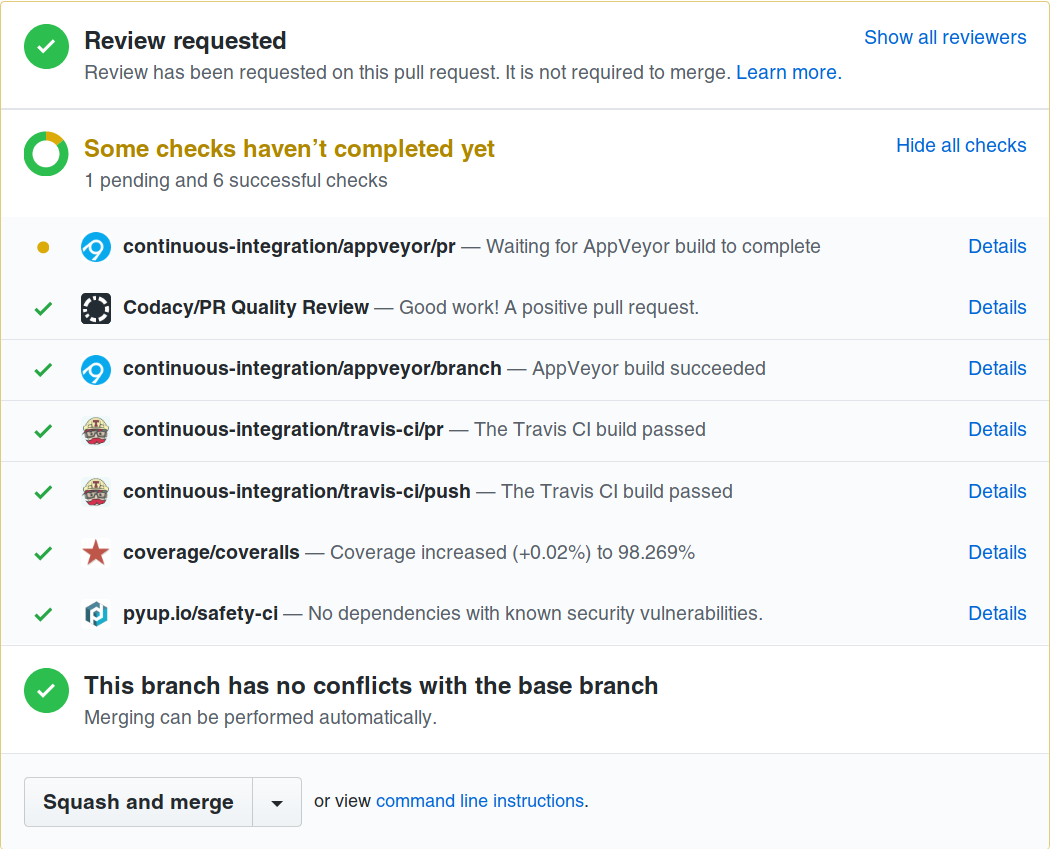
\includegraphics[width=.7\textwidth]{github_checks}
	\caption{Übersicht der durchlaufenden Checks}
	\label{github_checks}
\end{figure}

Die Unittests, welche von AppVeyor, Jenkins und Travis CI ausgeführt wurden, deckten große Teile des Python Codes ab. Sie sind im Github Repo
zu finden\footnote{\url{https://github.com/bp-flugsimulator/server/tree/master/frontend/tests}} und aufgrund ihrer Anzahl (~200) nicht
Teil des Anhangs.
Die Abdeckung lag immer bei über 90\% und war ein Kriterium für die Abnahme einer Userstory. Eine Übersicht der Abdeckung
findet sich in Abbildung \ref{coverage_pdf}.
Die Tests fanden unter folgenden Umgebungen statt:
\begin{itemize}
	\item Windows (Windows Server 2016, jeder Test mit 32 und 64 Bit Versionen)
		\begin{itemize}
			\item Python 3.4
			\item Python 3.5
			\item Python 3.6
		\end{itemize}
	\item Linux (Ubuntu, 64 Bit)
		\begin{itemize}
			\item Python 3.4
			\item Python 3.5
			\item Python 3.6
		\end{itemize}
\end{itemize}
\begin{figure}[t]
	\centering
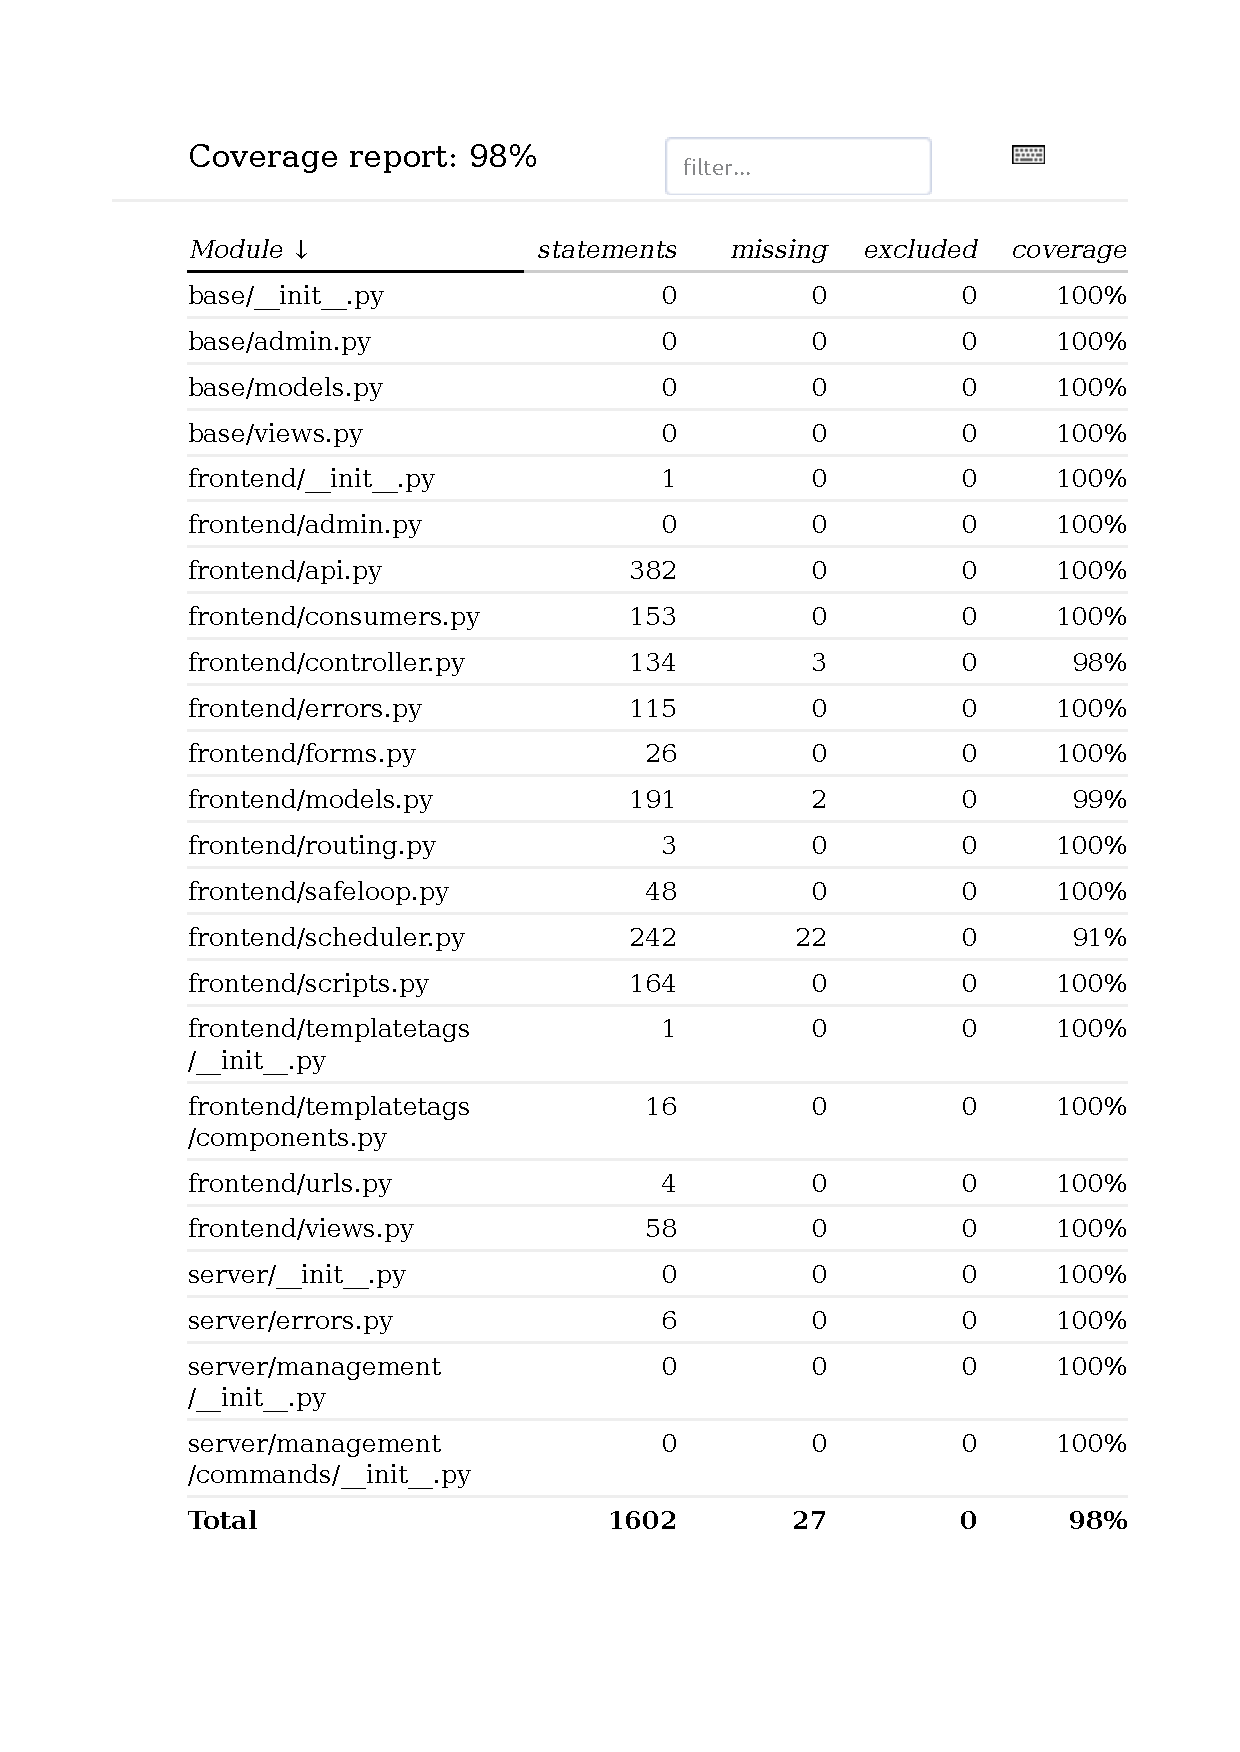
\includegraphics[width=.8\textwidth]{img/coverage.pdf}
	\caption{Abdeckungsübersicht am Ende des Projekts}
	\label{coverage_pdf}
\end{figure}
Der Stand von Codacy zum Ende des Projekts findet sich in Abbildung \ref{codacy_png}. Während
es keine stilistischen Fehler gibt ('Issues 0\%'), gibt es sehr viel doppelten Code, da viele Methoden
in der API einen ähnlichen bis gleichen Anfang haben.

\begin{longtable}{|p{10cm}|p{7cm}|}
\hline
Test Name & Klassenpfad (Prefix frontend.test wurd entfernt)\\\hline\hline
test\_entry\_delete\_deleted\_error & (test\_api.FilesystemTests)\\\hline
test\_entry\_delete\_not\_exist & (test\_api.FilesystemTests)\\\hline
test\_entry\_delete\_success & (test\_api.FilesystemTests)\\\hline
test\_entry\_post\_forbidden & (test\_api.FilesystemTests)\\\hline
test\_entry\_put\_exists & (test\_api.FilesystemTests)\\\hline
test\_entry\_put\_not\_exist & (test\_api.FilesystemTests)\\\hline
test\_entry\_put\_success & (test\_api.FilesystemTests)\\\hline
test\_entry\_put\_validation\_error & (test\_api.FilesystemTests)\\\hline
test\_move\_post\_conflict\_success & (test\_api.FilesystemTests)\\\hline
test\_move\_post\_exists\_error & (test\_api.FilesystemTests)\\\hline
test\_move\_post\_not\_exist & (test\_api.FilesystemTests)\\\hline
test\_move\_post\_offline & (test\_api.FilesystemTests)\\\hline
test\_move\_post\_offline\_error & (test\_api.FilesystemTests)\\\hline
test\_move\_post\_success & (test\_api.FilesystemTests)\\\hline
test\_move\_put\_forbidden & (test\_api.FilesystemTests)\\\hline
test\_restore\_post\_exists & (test\_api.FilesystemTests)\\\hline
test\_restore\_post\_not\_exist & (test\_api.FilesystemTests)\\\hline
test\_restore\_post\_offline & (test\_api.FilesystemTests)\\\hline
test\_restore\_post\_success & (test\_api.FilesystemTests)\\\hline
test\_restore\_put\_forbidden & (test\_api.FilesystemTests)\\\hline
test\_set\_delete\_forbidden & (test\_api.FilesystemTests)\\\hline
test\_set\_get\_query\_identifier\_error & (test\_api.FilesystemTests)\\\hline
test\_set\_get\_query\_not\_exist\_error & (test\_api.FilesystemTests)\\\hline
test\_set\_get\_query\_slaves\_success & (test\_api.FilesystemTests)\\\hline
test\_set\_get\_query\_success & (test\_api.FilesystemTests)\\\hline
test\_set\_post\_exist & (test\_api.FilesystemTests)\\\hline
test\_set\_post\_name\_error & (test\_api.FilesystemTests)\\\hline
test\_set\_post\_path\_error & (test\_api.FilesystemTests)\\\hline
test\_set\_post\_success & (test\_api.FilesystemTests)\\\hline
test\_set\_post\_validation\_error & (test\_api.FilesystemTests)\\\hline
test\_set\_post\_value\_error & (test\_api.FilesystemTests)\\\hline
test\_entry\_delete\_not\_exist & (test\_api.ProgramTests)\\\hline
test\_entry\_delete\_success & (test\_api.ProgramTests)\\\hline
test\_entry\_post\_forbidden & (test\_api.ProgramTests)\\\hline
test\_entry\_put\_exists & (test\_api.ProgramTests)\\\hline
test\_entry\_put\_not\_exist & (test\_api.ProgramTests)\\\hline
test\_entry\_put\_success & (test\_api.ProgramTests)\\\hline
test\_entry\_put\_validation\_error & (test\_api.ProgramTests)\\\hline
test\_log\_disable\_delete\_forbidden & (test\_api.ProgramTests)\\\hline
test\_log\_disable\_post\_not\_exist & (test\_api.ProgramTests)\\\hline
test\_log\_disable\_post\_offline & (test\_api.ProgramTests)\\\hline
test\_log\_disable\_post\_success & (test\_api.ProgramTests)\\\hline
test\_log\_enable\_delete\_forbidden & (test\_api.ProgramTests)\\\hline
test\_log\_enable\_post\_not\_exist & (test\_api.ProgramTests)\\\hline
test\_log\_enable\_post\_offline\_error & (test\_api.ProgramTests)\\\hline
test\_log\_enable\_post\_success & (test\_api.ProgramTests)\\\hline
test\_log\_entry\_delete\_forbidden & (test\_api.ProgramTests)\\\hline
test\_log\_entry\_get\_not\_exist & (test\_api.ProgramTests)\\\hline
test\_log\_entry\_get\_success & (test\_api.ProgramTests)\\\hline
test\_set\_delete\_query\_forbidden & (test\_api.ProgramTests)\\\hline
test\_set\_get\_query\_identifier\_error & (test\_api.ProgramTests)\\\hline
test\_set\_get\_query\_not\_exist\_error & (test\_api.ProgramTests)\\\hline
test\_set\_get\_query\_slaves\_success & (test\_api.ProgramTests)\\\hline
test\_set\_get\_query\_success & (test\_api.ProgramTests)\\\hline
test\_set\_post\_success & (test\_api.ProgramTests)\\\hline
test\_set\_post\_too\_long\_error & (test\_api.ProgramTests)\\\hline
test\_set\_post\_value\_error & (test\_api.ProgramTests)\\\hline
test\_start\_delete\_forbidden & (test\_api.ProgramTests)\\\hline
test\_start\_post\_exist & (test\_api.ProgramTests)\\\hline
test\_start\_post\_not\_exist & (test\_api.ProgramTests)\\\hline
test\_start\_post\_offline & (test\_api.ProgramTests)\\\hline
test\_start\_post\_success & (test\_api.ProgramTests)\\\hline
test\_stop\_delete\_forbidden & (test\_api.ProgramTests)\\\hline
test\_stop\_post\_not\_exist & (test\_api.ProgramTests)\\\hline
test\_stop\_post\_not\_running\_error & (test\_api.ProgramTests)\\\hline
test\_stop\_post\_offline & (test\_api.ProgramTests)\\\hline
test\_stop\_post\_success & (test\_api.ProgramTests)\\\hline
test\_copy\_delete\_forbidden & (test\_api.ScriptTest)\\\hline
test\_copy\_post\_not\_exist & (test\_api.ScriptTest)\\\hline
test\_copy\_post\_success & (test\_api.ScriptTest)\\\hline
test\_entry\_delete\_not\_exist & (test\_api.ScriptTest)\\\hline
test\_entry\_delete\_success & (test\_api.ScriptTest)\\\hline
test\_entry\_get\_not\_exist & (test\_api.ScriptTest)\\\hline
test\_entry\_get\_query\_filesystem\_success & (test\_api.ScriptTest)\\\hline
test\_entry\_get\_query\_parameter\_error & (test\_api.ScriptTest)\\\hline
test\_entry\_get\_query\_programs\_success & (test\_api.ScriptTest)\\\hline
test\_entry\_get\_query\_slaves\_success & (test\_api.ScriptTest)\\\hline
test\_entry\_get\_success & (test\_api.ScriptTest)\\\hline
test\_entry\_get\_type\_error & (test\_api.ScriptTest)\\\hline
test\_entry\_post\_forbidden & (test\_api.ScriptTest)\\\hline
test\_entry\_put\_exist & (test\_api.ScriptTest)\\\hline
test\_entry\_put\_success & (test\_api.ScriptTest)\\\hline
test\_run\_post\_not\_exist & (test\_api.ScriptTest)\\\hline
test\_run\_post\_running\_error & (test\_api.ScriptTest)\\\hline
test\_run\_put\_forbidden & (test\_api.ScriptTest)\\\hline
test\_set\_default\_forbidden & (test\_api.ScriptTest)\\\hline
test\_set\_default\_success & (test\_api.ScriptTest)\\\hline
test\_set\_post\_key\_error & (test\_api.ScriptTest)\\\hline
test\_set\_post\_negtaive\_index\_error & (test\_api.ScriptTest)\\\hline
test\_set\_post\_not\_exist & (test\_api.ScriptTest)\\\hline
test\_set\_post\_success & (test\_api.ScriptTest)\\\hline
test\_set\_post\_type\_error & (test\_api.ScriptTest)\\\hline
test\_set\_post\_unique\_error & (test\_api.ScriptTest)\\\hline
test\_set\_post\_value\_error & (test\_api.ScriptTest)\\\hline
test\_set\_put\_forbidden & (test\_api.ScriptTest)\\\hline
test\_stop\_post\_success & (test\_api.ScriptTest)\\\hline
test\_stop\_put\_forbidden & (test\_api.ScriptTest)\\\hline
test\_entry\_delete\_not\_exist & (test\_api.SlaveTests)\\\hline
test\_entry\_delete\_success & (test\_api.SlaveTests)\\\hline
test\_entry\_get\_forbidden & (test\_api.SlaveTests)\\\hline
test\_entry\_get\_offline\_slave & (test\_api.SlaveTests)\\\hline
test\_entry\_put\_exist & (test\_api.SlaveTests)\\\hline
test\_entry\_put\_not\_exist & (test\_api.SlaveTests)\\\hline
test\_entry\_put\_success & (test\_api.SlaveTests)\\\hline
test\_entry\_put\_unique\_error & (test\_api.SlaveTests)\\\hline
test\_entry\_put\_value\_error & (test\_api.SlaveTests)\\\hline
test\_set\_delete\_forbidden & (test\_api.SlaveTests)\\\hline
test\_set\_get\_query\_filesystem\_success & (test\_api.SlaveTests)\\\hline
test\_set\_get\_query\_programs\_success & (test\_api.SlaveTests)\\\hline
test\_set\_get\_query\_simultaneous\_error & (test\_api.SlaveTests)\\\hline
test\_set\_get\_query\_success & (test\_api.SlaveTests)\\\hline
test\_set\_post\_success & (test\_api.SlaveTests)\\\hline
test\_shutdown\_delete\_forbidden & (test\_api.SlaveTests)\\\hline
test\_shutdown\_post\_not\_exist & (test\_api.SlaveTests)\\\hline
test\_shutdown\_post\_offline & (test\_api.SlaveTests)\\\hline
test\_shutdown\_post\_success & (test\_api.SlaveTests)\\\hline
test\_stop\_all\_post\_success & (test\_api.SlaveTests)\\\hline
test\_stop\_all\_put\_forbidden & (test\_api.SlaveTests)\\\hline
test\_wol\_delete\_forbidden & (test\_api.SlaveTests)\\\hline
test\_wol\_post\_not\_exist & (test\_api.SlaveTests)\\\hline
test\_wol\_post\_success & (test\_api.SlaveTests)\\\hline
test\_script\_entry & (test\_components.ComponentTests)\\\hline
test\_argument\_validator\_list & (test\_database.DatabaseTests)\\\hline
test\_argument\_validator\_list\_raises & (test\_database.DatabaseTests)\\\hline
test\_filesystem\_state & (test\_database.DatabaseTests)\\\hline
test\_filesystem\_str & (test\_database.DatabaseTests)\\\hline
test\_flush\_error & (test\_database.DatabaseTests)\\\hline
test\_flush\_success & (test\_database.DatabaseTests)\\\hline
test\_mac\_validator\_lower & (test\_database.DatabaseTests)\\\hline
test\_mac\_validator\_mixed & (test\_database.DatabaseTests)\\\hline
test\_mac\_validator\_too\_long & (test\_database.DatabaseTests)\\\hline
test\_mac\_validator\_too\_long\_inner & (test\_database.DatabaseTests)\\\hline
test\_mac\_validator\_too\_short & (test\_database.DatabaseTests)\\\hline
test\_mac\_validator\_too\_short\_inner & (test\_database.DatabaseTests)\\\hline
test\_mac\_validator\_upper & (test\_database.DatabaseTests)\\\hline
test\_program\_error & (test\_database.DatabaseTests)\\\hline
test\_program\_is\_err & (test\_database.DatabaseTests)\\\hline
test\_program\_is\_timeouted & (test\_database.DatabaseTests)\\\hline
test\_program\_running & (test\_database.DatabaseTests)\\\hline
test\_program\_state & (test\_database.DatabaseTests)\\\hline
test\_program\_successful & (test\_database.DatabaseTests)\\\hline
test\_reset\_success & (test\_database.DatabaseTests)\\\hline
test\_script\_check\_online & (test\_database.DatabaseTests)\\\hline
test\_script\_has\_error & (test\_database.DatabaseTests)\\\hline
test\_script\_indexes & (test\_database.DatabaseTests)\\\hline
test\_script\_last\_ran & (test\_database.DatabaseTests)\\\hline
test\_script\_latest & (test\_database.DatabaseTests)\\\hline
test\_script\_name & (test\_database.DatabaseTests)\\\hline
test\_script\_stages & (test\_database.DatabaseTests)\\\hline
test\_slave\_data\_state & (test\_database.DatabaseTests)\\\hline
test\_slave\_has\_err & (test\_database.DatabaseTests)\\\hline
test\_slave\_has\_error\_true & (test\_database.DatabaseTests)\\\hline
test\_slave\_insert\_invalid\_ip & (test\_database.DatabaseTests)\\\hline
test\_slave\_insert\_invalid\_mac & (test\_database.DatabaseTests)\\\hline
test\_slave\_is\_online\_err & (test\_database.DatabaseTests)\\\hline
test\_download\_page\_0\_byte & (test\_download.DownloadTests)\\\hline
test\_download\_page\_1\_gib & (test\_download.DownloadTests)\\\hline
test\_download\_page\_1\_kib & (test\_download.DownloadTests)\\\hline
test\_download\_page\_1\_mib & (test\_download.DownloadTests)\\\hline
test\_download\_page\_no\_folder & (test\_download.DownloadTests)\\\hline
test\_filesystem\_base & (test\_errors.BaseErrorTests)\\\hline
test\_program\_base & (test\_errors.BaseErrorTests)\\\hline
test\_query\_base & (test\_errors.BaseErrorTests)\\\hline
test\_script\_base & (test\_errors.BaseErrorTests)\\\hline
test\_download\_page\_0\_byte & (test\_frontend.DownloadTests)\\\hline
test\_download\_page\_1\_gib & (test\_frontend.DownloadTests)\\\hline
test\_download\_page\_1\_kib & (test\_frontend.DownloadTests)\\\hline
test\_download\_page\_1\_mib & (test\_frontend.DownloadTests)\\\hline
test\_download\_page\_no\_folder & (test\_frontend.DownloadTests)\\\hline
test\_run\_script\_get & (test\_frontend.FrontendTests)\\\hline
test\_scripts\_get & (test\_frontend.FrontendTests)\\\hline
test\_slave\_get & (test\_frontend.FrontendTests)\\\hline
test\_slave\_get\_empty & (test\_frontend.FrontendTests)\\\hline
test\_welcome\_get & (test\_frontend.FrontendTests)\\\hline
test\_file\_slave\_not\_exist\_error & (test\_script.ScriptTests)\\\hline
test\_from\_json & (test\_script.ScriptTests)\\\hline
test\_from\_json\_file & (test\_script.ScriptTests)\\\hline
test\_from\_json\_program & (test\_script.ScriptTests)\\\hline
test\_from\_query\_error & (test\_script.ScriptTests)\\\hline
test\_get\_slave\_int & (test\_script.ScriptTests)\\\hline
test\_get\_slave\_int\_not\_found & (test\_script.ScriptTests)\\\hline
test\_get\_slave\_none & (test\_script.ScriptTests)\\\hline
test\_get\_slave\_str & (test\_script.ScriptTests)\\\hline
test\_get\_slave\_str\_not\_found & (test\_script.ScriptTests)\\\hline
test\_integer\_identifiers & (test\_script.ScriptTests)\\\hline
test\_model\_references\_same\_int & (test\_script.ScriptTests)\\\hline
test\_model\_references\_same\_str & (test\_script.ScriptTests)\\\hline
test\_name\_not\_equal & (test\_script.ScriptTests)\\\hline
test\_positive\_index\_error & (test\_script.ScriptTests)\\\hline
test\_program\_not\_exist & (test\_script.ScriptTests)\\\hline
test\_program\_slave\_not\_exist\_error & (test\_script.ScriptTests)\\\hline
test\_string\_identifiers & (test\_script.ScriptTests)\\\hline
test\_connect\_and\_disconnect\_success & (test\_websockets.LogWebsocketTests)\\\hline
test\_connect\_and\_disconnect\_success & (test\_websockets.NotificationWebsocketTests)\\\hline
test\_connect\_slave\_not\_exists & (test\_websockets.RPCWebsocketTests)\\\hline
test\_connect\_success & (test\_websockets.RPCWebsocketTests)\\\hline
test\_disconnect\_slave\_not\_exists & (test\_websockets.RPCWebsocketTests)\\\hline
test\_disconnect\_success & (test\_websockets.RPCWebsocketTests)\\\hline
test\_rceive\_filesystem\_moved\_filesystem\_not\_exists & (test\_websockets.RPCWebsocketTests)\\\hline
test\_receive\_chain\_commands\_success & (test\_websockets.RPCWebsocketTests)\\\hline
test\_receive\_chain\_commands\_with\_error\_status & (test\_websockets.RPCWebsocketTests)\\\hline
test\_receive\_execute\_slave\_not\_exists & (test\_websockets.RPCWebsocketTests)\\\hline
test\_receive\_execute\_success & (test\_websockets.RPCWebsocketTests)\\\hline
test\_receive\_execute\_with\_error\_status & (test\_websockets.RPCWebsocketTests)\\\hline
test\_receive\_filesystem\_moved\_success & (test\_websockets.RPCWebsocketTests)\\\hline
test\_receive\_filesystem\_moved\_with\_error\_code & (test\_websockets.RPCWebsocketTests)\\\hline
test\_receive\_filesystem\_restore\_filesystem\_not\_exists & (test\_websockets.RPCWebsocketTests)\\\hline
test\_receive\_filesystem\_restore\_success & (test\_websockets.RPCWebsocketTests)\\\hline
test\_receive\_filesystem\_restore\_with\_error\_code & (test\_websockets.RPCWebsocketTests)\\\hline
test\_receive\_get\_log\_program\_not\_exists & (test\_websockets.RPCWebsocketTests)\\\hline
test\_receive\_get\_log\_success & (test\_websockets.RPCWebsocketTests)\\\hline
test\_receive\_get\_log\_with\_error\_status & (test\_websockets.RPCWebsocketTests)\\\hline
test\_receive\_no\_content & (test\_websockets.RPCWebsocketTests)\\\hline
test\_receive\_online\_slave\_not\_exists & (test\_websockets.RPCWebsocketTests)\\\hline
test\_receive\_online\_success & (test\_websockets.RPCWebsocketTests)\\\hline
test\_receive\_online\_with\_error\_status & (test\_websockets.RPCWebsocketTests)\\\hline
test\_receive\_parse\_json & (test\_websockets.RPCWebsocketTests)\\\hline
test\_receive\_unknown\_message\_type & (test\_websockets.RPCWebsocketTests)\\\hline
test\_start & (test\_scheduler.SchedulerTests)\\\hline
test\_state\_error & (test\_scheduler.SchedulerTests)\\\hline
test\_state\_init & (test\_scheduler.SchedulerTests)\\\hline
test\_state\_next & (test\_scheduler.SchedulerTests)\\\hline
test\_state\_next\_finished & (test\_scheduler.SchedulerTests)\\\hline
test\_state\_next\_finished\_filesystem & (test\_scheduler.SchedulerTests)\\\hline
test\_state\_next\_offline\_filesystem & (test\_scheduler.SchedulerTests)\\\hline
test\_state\_next\_offline\_program & (test\_scheduler.SchedulerTests)\\\hline
test\_state\_success & (test\_scheduler.SchedulerTests)\\\hline
test\_state\_waiting\_filesystems\_error & (test\_scheduler.SchedulerTests)\\\hline
test\_state\_waiting\_programs\_error & (test\_scheduler.SchedulerTests)\\\hline
test\_state\_waiting\_programs\_success & (test\_scheduler.SchedulerTests)\\\hline
test\_state\_waiting\_slaves & (test\_scheduler.SchedulerTests)\\\hline
test\_stop & (test\_scheduler.SchedulerTests)\\\hline
test\_timer\_slave\_timeout & (test\_scheduler.SchedulerTests)\\\hline
\end{longtable}

Ein erfolgreicher Testrun von Travis\footnote{\url{https://travis-ci.org/bp-flugsimulator}} ist in Abbildung \ref{travis_png} zu sehen, von AppVeyor\footnote{\url{https://ci.appveyor.com/project/GreenM0nst3r/server/history}} in Abbildung \ref{appveyor_png}.
Die Ergebnisse finden sich unter 


\begin{figure}[t]
	\centering
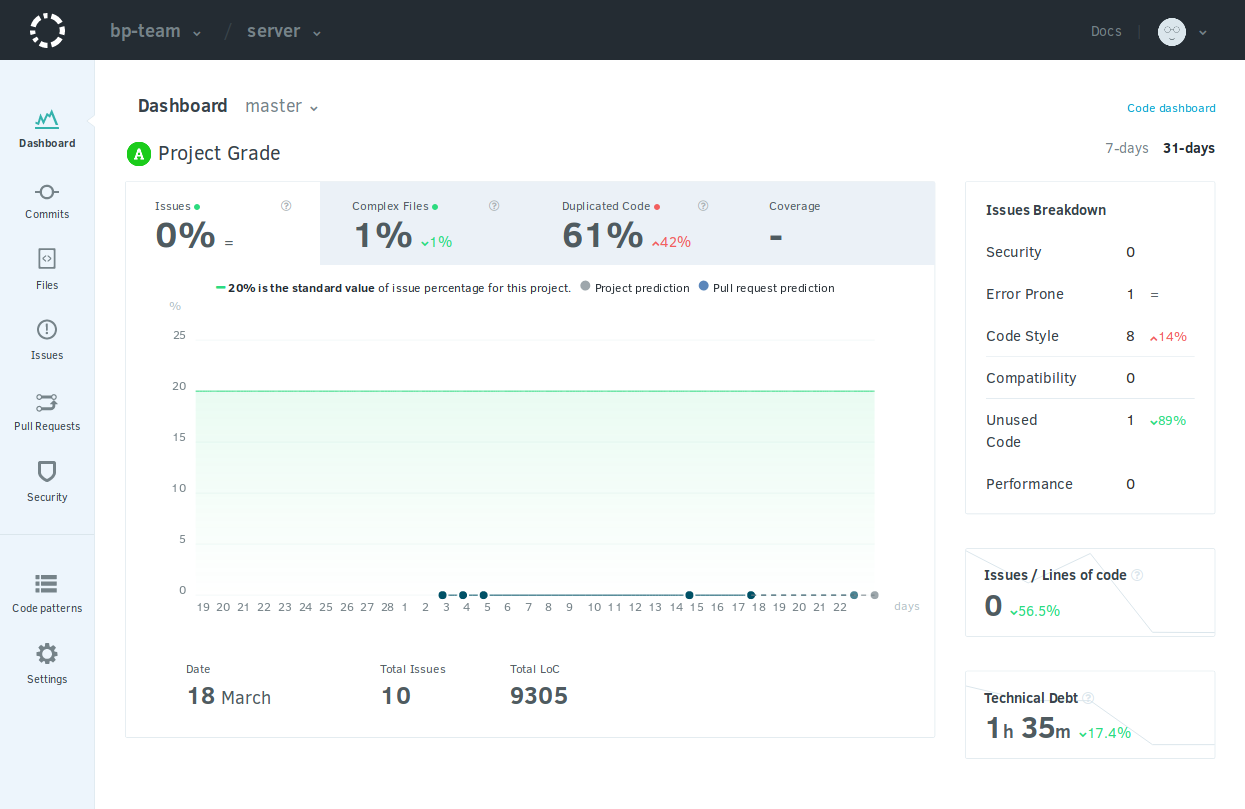
\includegraphics[width=.9\textwidth]{codacy}
	\caption{Stilüberprüfung am Ende des Projekts}
	\label{codacy_png}
\end{figure}

\begin{figure}[h]
	\centering
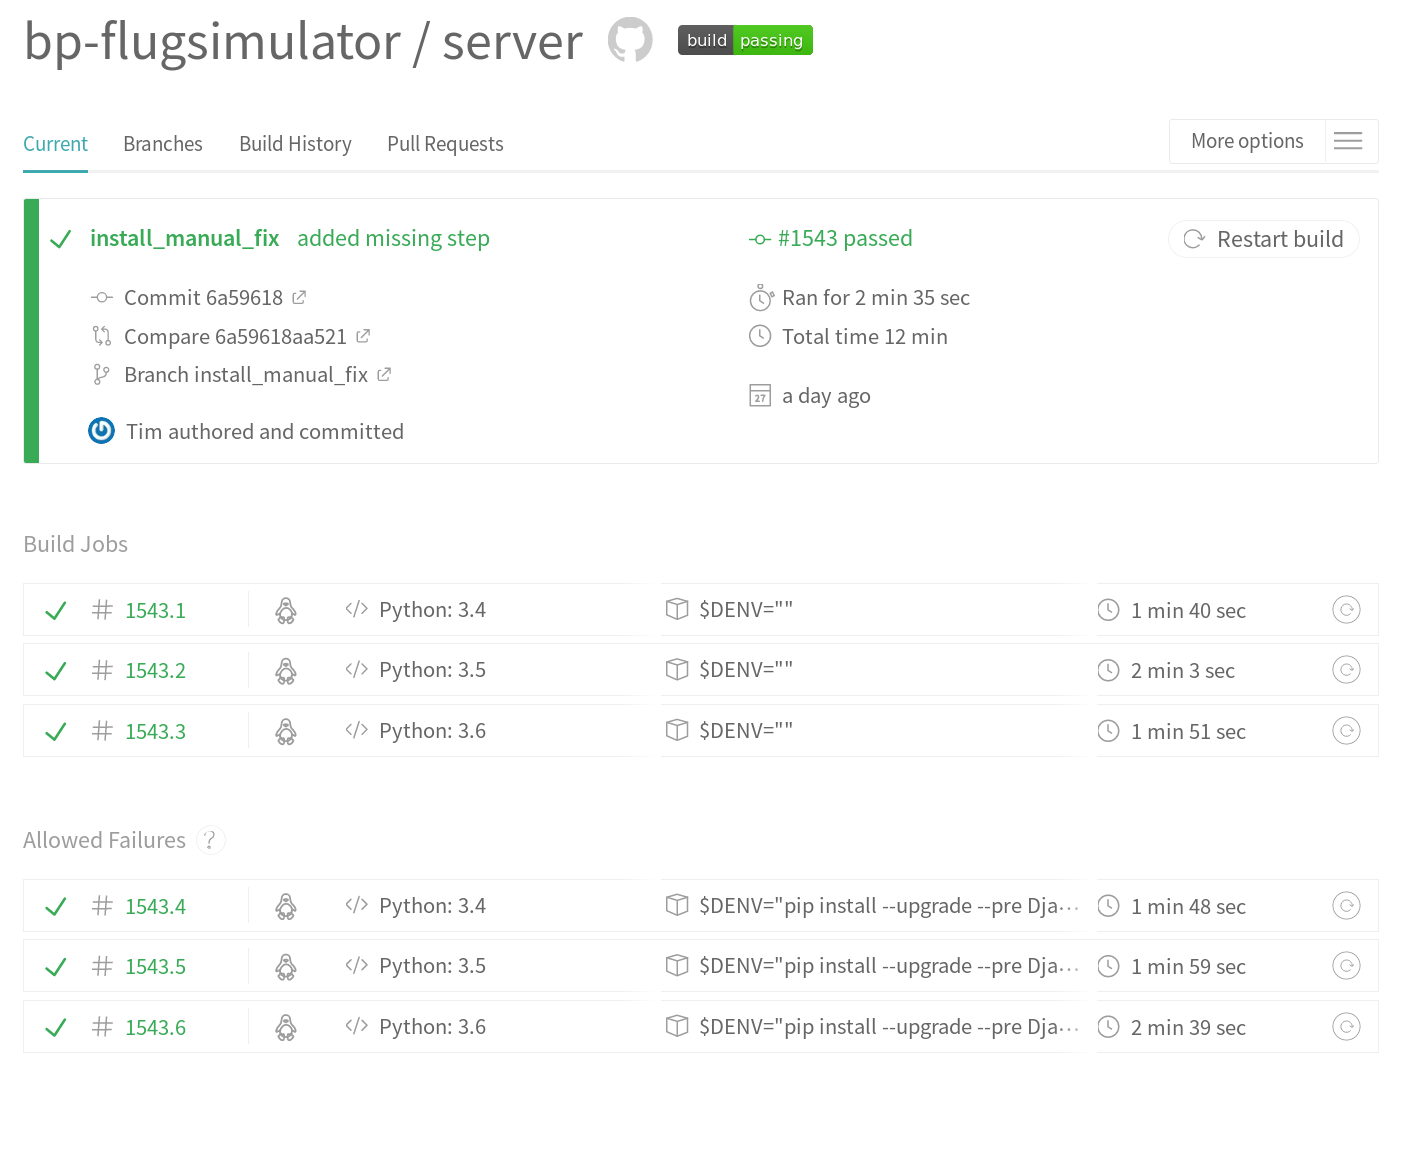
\includegraphics[width=.9\textwidth]{travis}
	\caption{Erfolgreicher Testdurchlauf von Travis}
	\label{travis_png}
\end{figure}

\begin{figure}[h]
	\centering
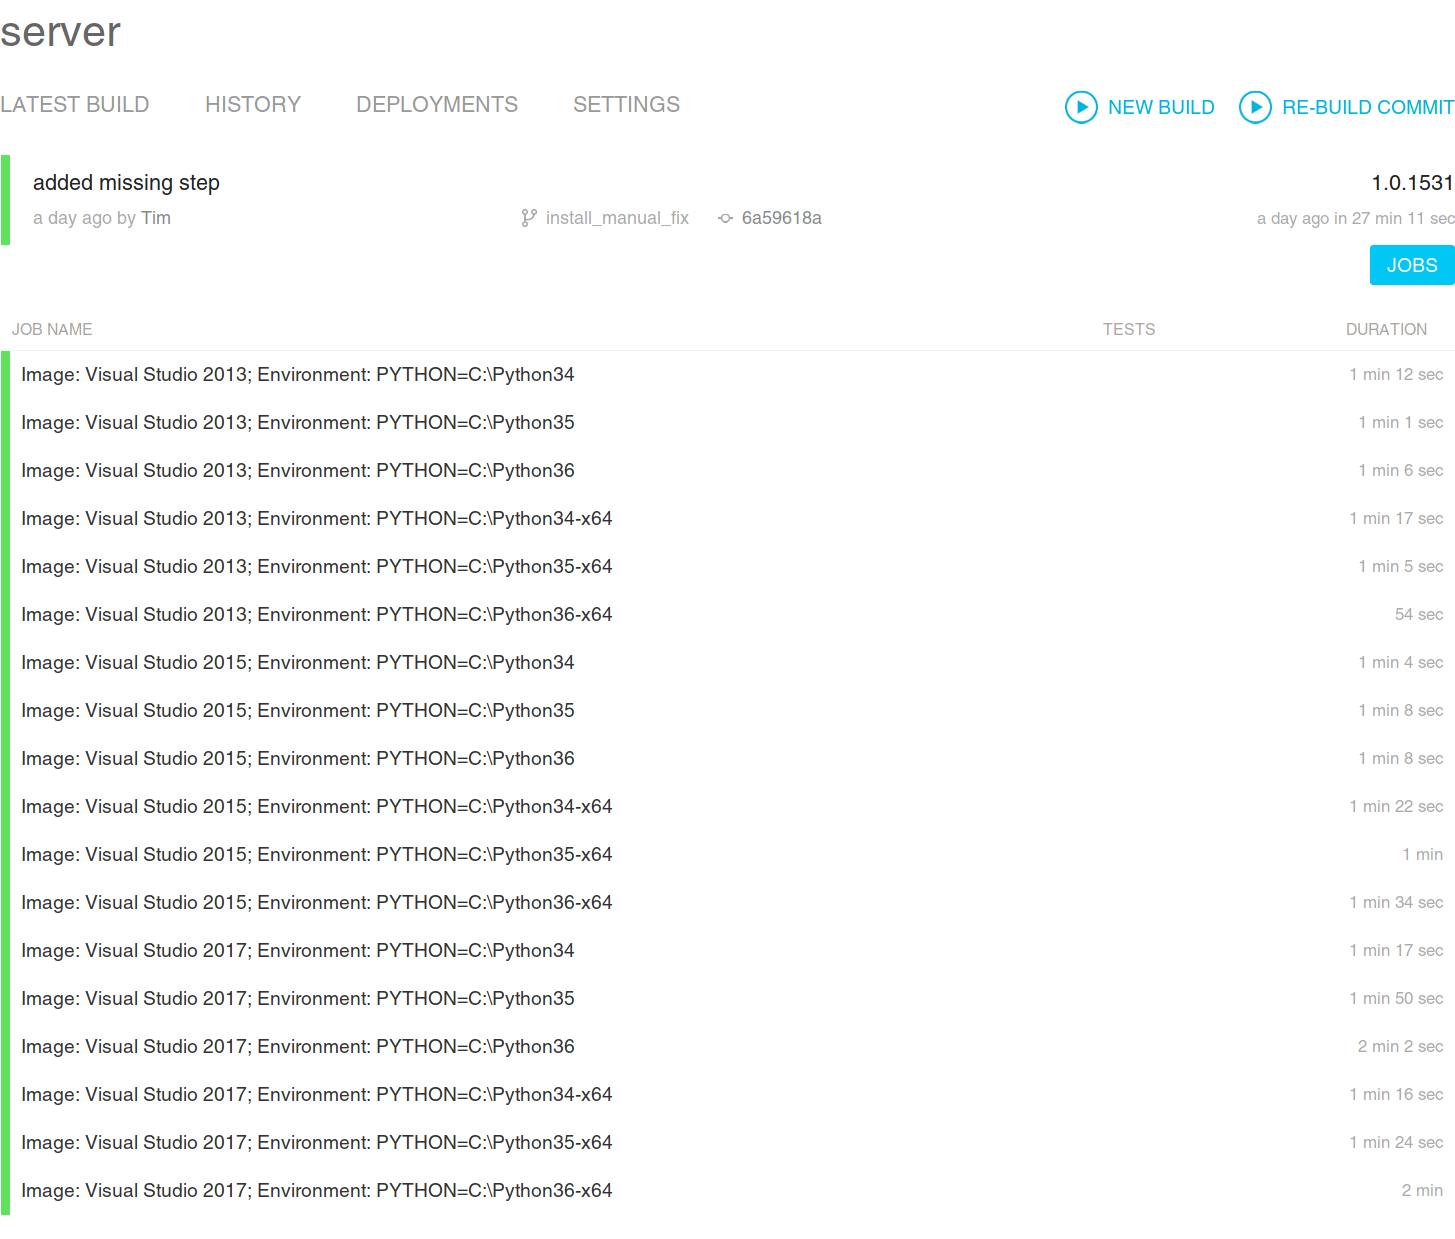
\includegraphics[width=.9\textwidth]{appveyor}
	\caption{Erfolgreicher Testdurchlauf von AppVeyor}
	\label{appveyor_png}
\end{figure}

\begin{figure}[h]
	\centering
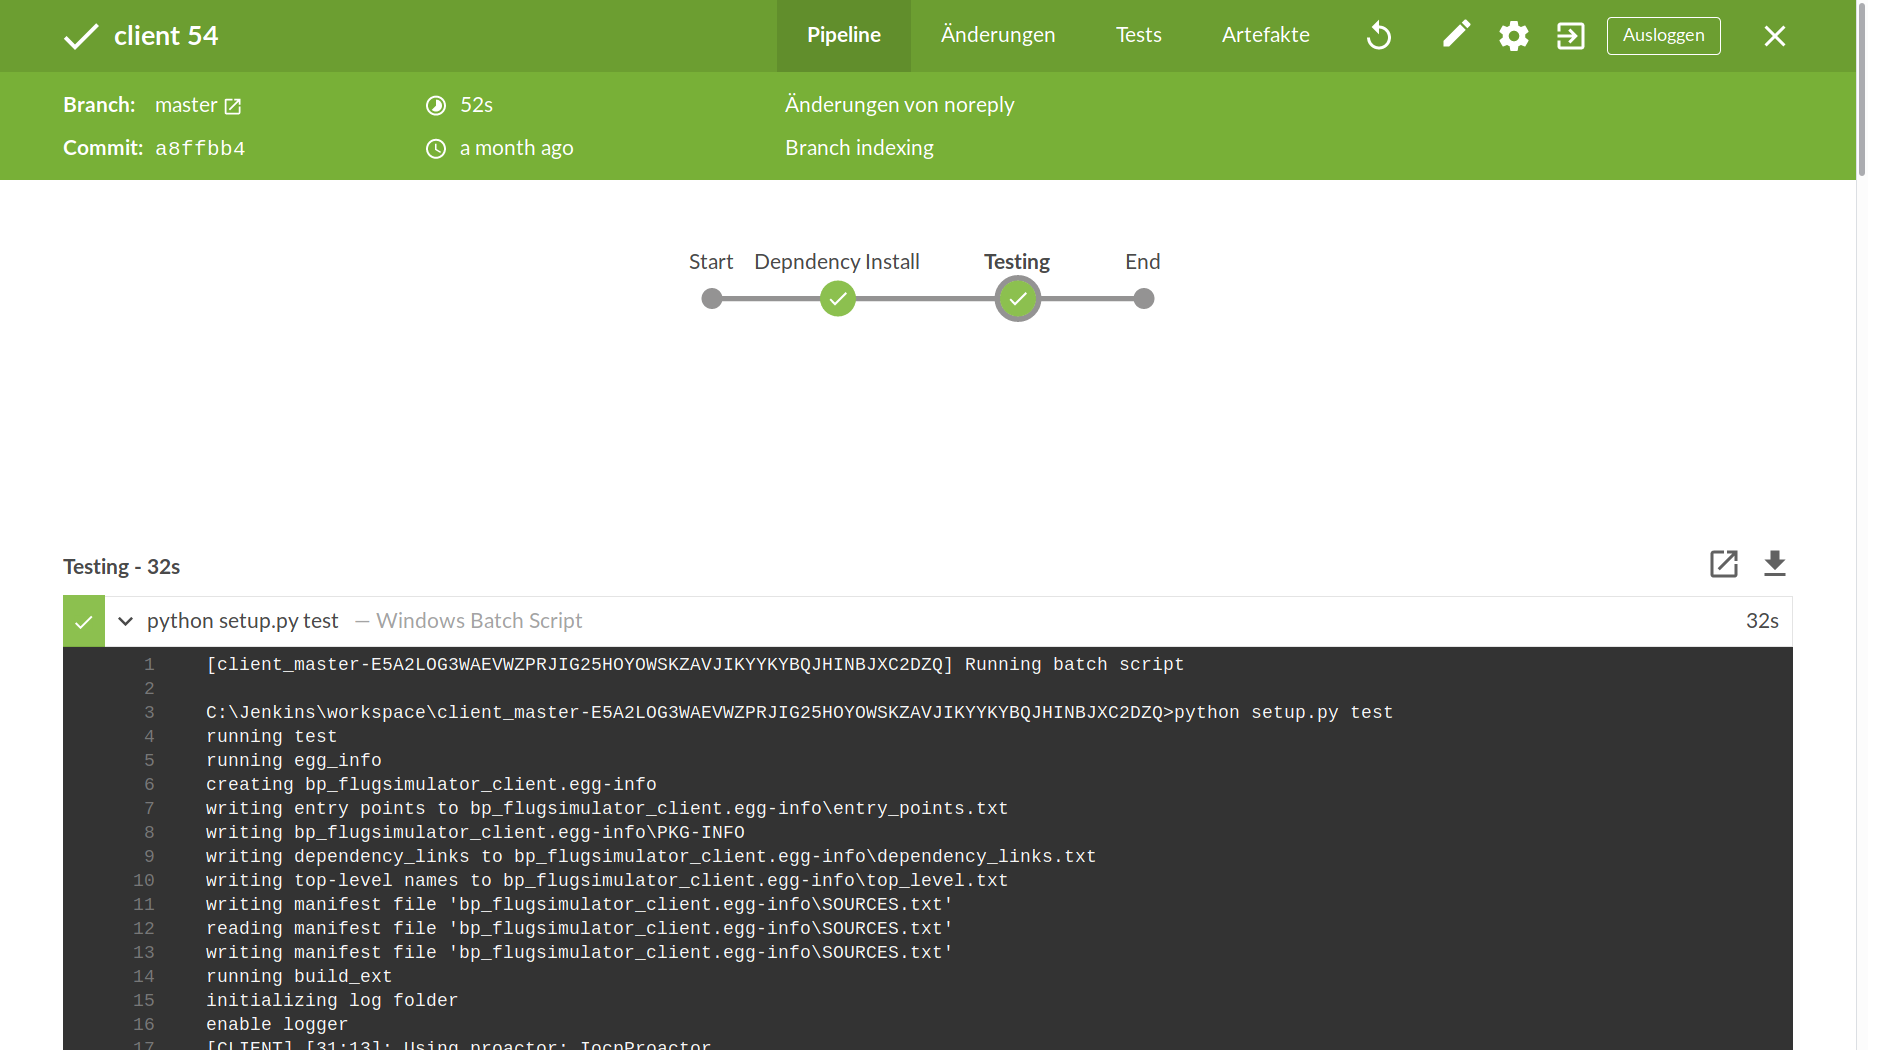
\includegraphics[width=.8\textwidth]{img/jenkins.png}
	\caption{Erfolgreicher Testdurchlauf von jenkins}
	\label{jenkins_png}
\end{figure}

	% Details zu den Iterationen
	\section{QS-Prozess nach Iteration}
So wie das Projekt ist auch der QS-Prozess im Projektverlauf angewachsen. Es wurden neue Tools hinzugefügt
und neue Testumgebungen entwickelt, da die Auftraggeber ihre Anforderungen geändert haben. Daher gibt
es nicht für alle Iterationen vollständige Testausgaben. Zudem haben einige Tools (AppVeyor und Travis CI)
die gleichen Tests durchgeführt. Dort wurde dann nur ein Output angehängt.

Die Iterationslänge betrug zwei Wochen.

\subsubsection{1. Iteration}
\begin{table}[H]
\begin{center}
	\begin{tabular}{| l | l |}
		\hline
		\textbf{Zeitraum} & 13.11.2017 - 26.11.2017\\\hline
		\textbf{Abgegebene Userstorys} & 1, 2, 6, 14, 15, 16 \\\hline
		\textbf{Commit Hash} & \texttt{f3bbc82b0eb9ef5c0159843152fc54fb7c5c8309} \\\hline
	\end{tabular}
	\caption{Übersicht 1. Iteration}
\end{center}
\end{table}

\subsubsection{Testoutput (\texttt{python manage.py test})}
\lstinputlisting{test_output/01_iteration_python}

\subsubsection{2. Iteration}
\begin{table}[H]
\begin{center}
	\begin{tabular}{| l | l |}
		\hline
		\textbf{Zeitraum} & 27.11.2017 - 10.12.2017\\\hline
		\textbf{Abgegebene Userstorys} & 3, 19, 20, 21\\\hline
		\textbf{Commit Hash} & \texttt{eef5badcf7928d55461bfddb40c3f7f7194a0fa3} \\\hline
	\end{tabular}
	\caption{Übersicht 2. Iteration}
\end{center}
\end{table}
\subsubsection{Testoutput (\texttt{python manage.py test})}
\lstinputlisting{test_output/02_iteration_python}

\subsubsection{3. Iteration}
\begin{table}[H]
\begin{center}
	\begin{tabular}{| l | l |}
		\hline
		\textbf{Zeitraum} & 11.12.2017 - 07.01.2018\\\hline
		\textbf{Abgegebene Userstorys} & 5, 7, 17, 22, 23, 24, 27\\\hline
		\textbf{Commit Hash} & \texttt{b5c84ab3496ade220316b8b119c7fddc3d49d383} \\\hline
	\end{tabular}
	\caption{Übersicht 3. Iteration}
\end{center}
\end{table}
\subsubsection{Testoutput (\texttt{python manage.py test})}
\lstinputlisting{test_output/03_iteration_python}
\subsubsection{Coverage}
\begin{figure}[H]
	\centering
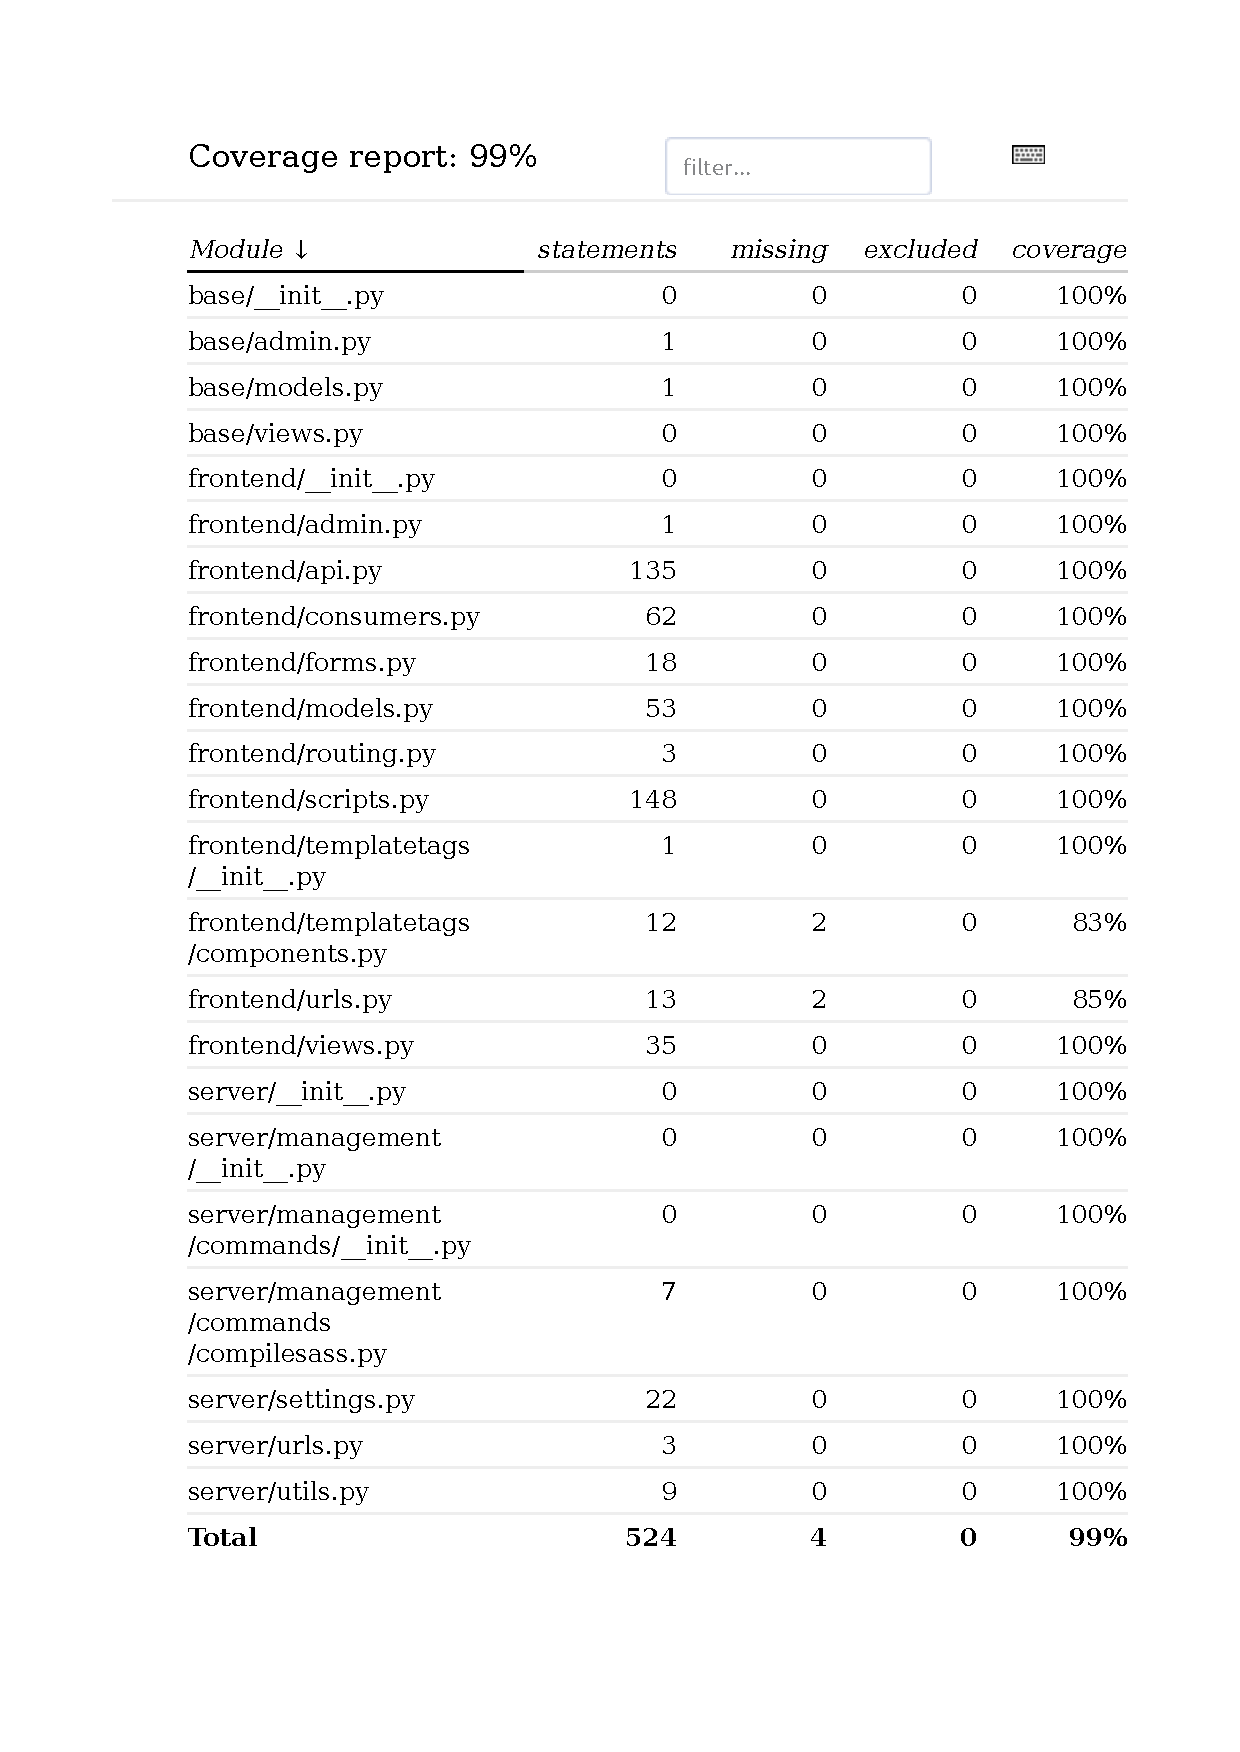
\includegraphics[width=.9\textwidth]{test_output/03_iteration_coverage.pdf}
	\caption{Coverage in Iteration 3}
\end{figure}

\subsubsection{4. Iteration}
\begin{table}[H]
\begin{center}
	\begin{tabular}{| l | l |}
		\hline
		\textbf{Zeitraum} & 08.01.2018 - 21.01.2018\\\hline
		\textbf{Abgegebene Userstorys} & 4, 8, 28, 29, 33, 34, 35, 36, \\\hline
		\textbf{Commit Hash} & \texttt{b06b3f8b23a022a127061c2dae05215c0bc21f23} \\\hline
	\end{tabular}
	\caption{Übersicht 4. Iteration}
\end{center}
\end{table}
\subsubsection{Testoutput (\texttt{python manage.py test})}
\lstinputlisting{test_output/04_iteration_python}
\subsubsection{Coverage}
\begin{figure}[H]
	\centering
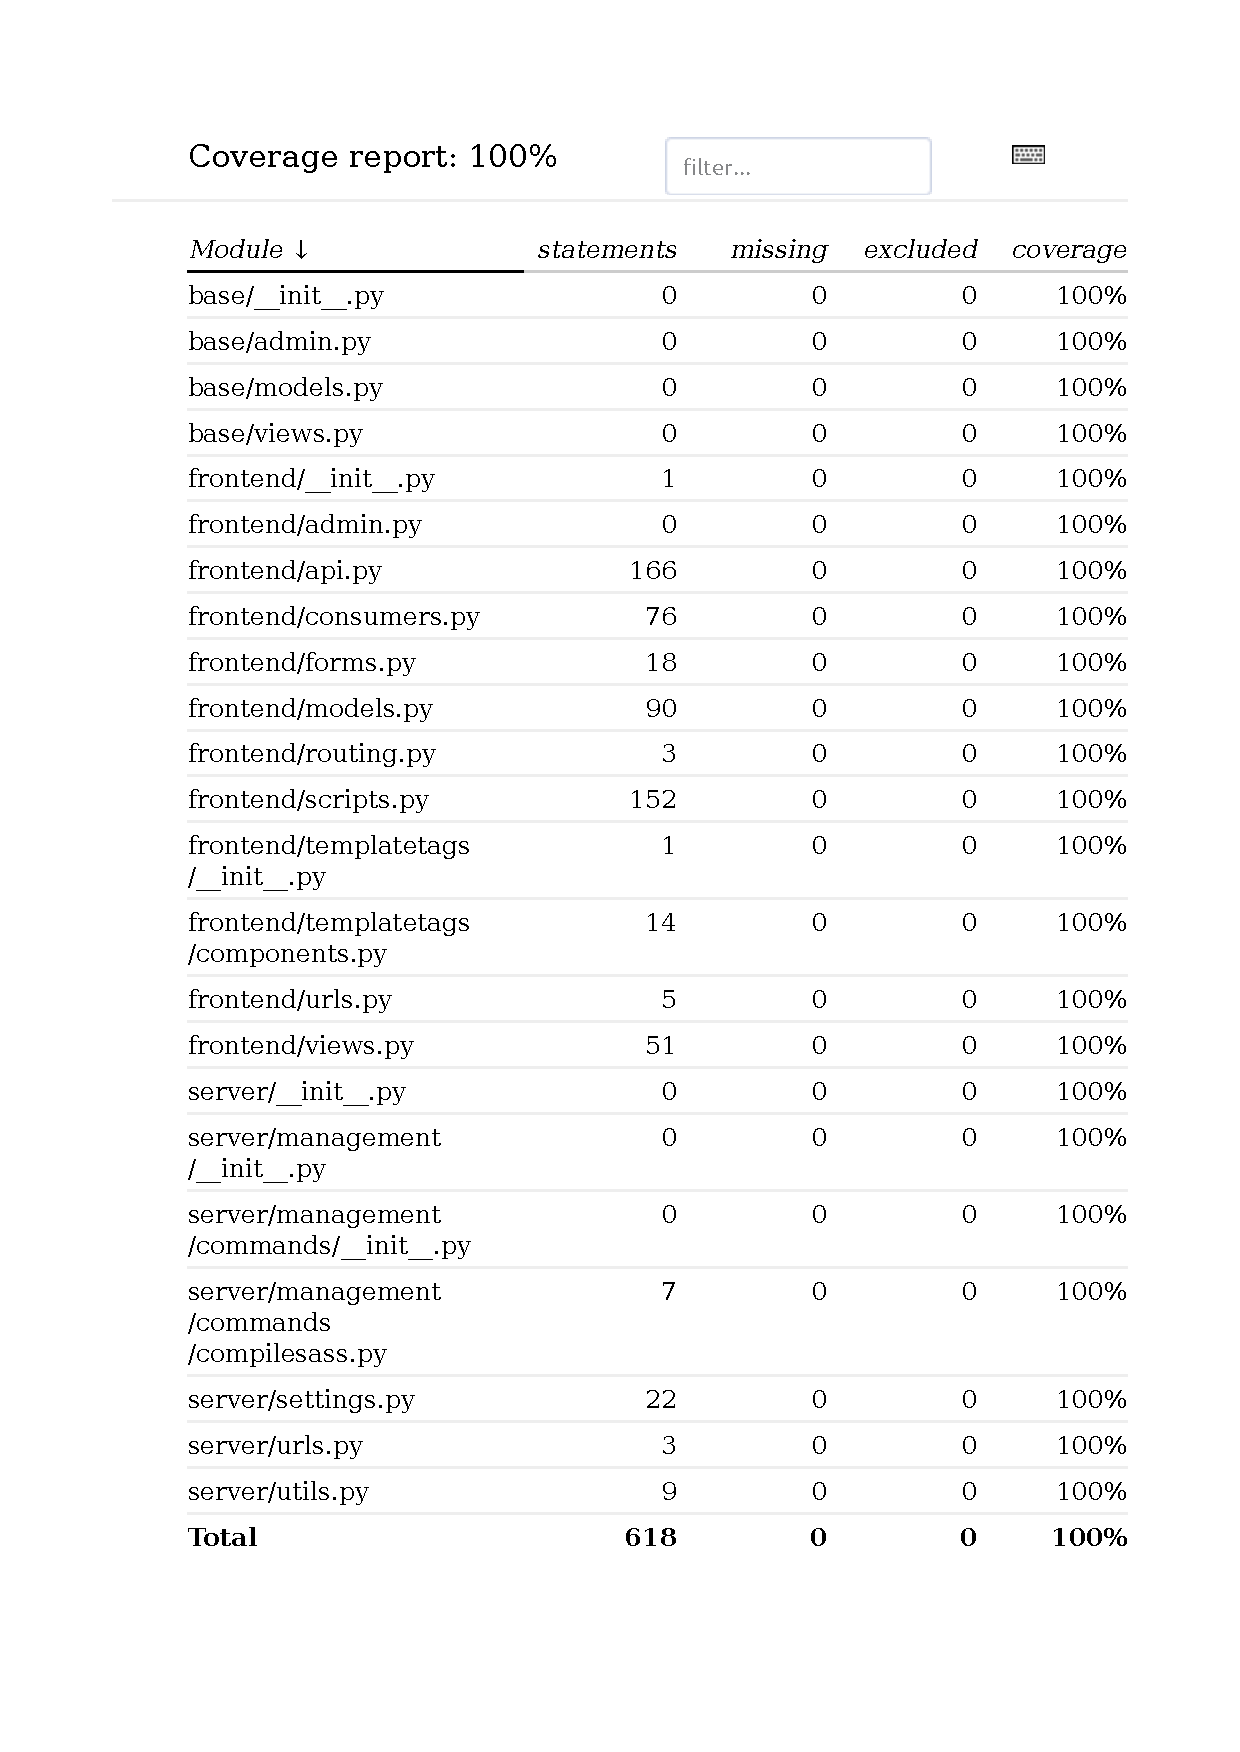
\includegraphics[width=.9\textwidth]{test_output/04_iteration_coverage.pdf}
	\caption{Coverage in Iteration 4}
\end{figure}

\subsubsection{5. Iteration}
\begin{table}[H]
\begin{center}
	\begin{tabular}{| l | l |}
		\hline
		\textbf{Zeitraum} &  22.01.2018 - 04.02.2018\\\hline
		\textbf{Abgegebene Userstorys} & 25, 31\\\hline
		\textbf{Commit Hash} & \texttt{8a194372e807cc043f3ea705671d515fd0fe0bb5} \\\hline
	\end{tabular}
	\caption{Übersicht 5. Iteration}
\end{center}
\end{table}
\subsubsection{Testoutput }
\lstinputlisting{test_output/05_iteration_python}
\subsubsection{Coverage}
\begin{figure}[H]
	\centering
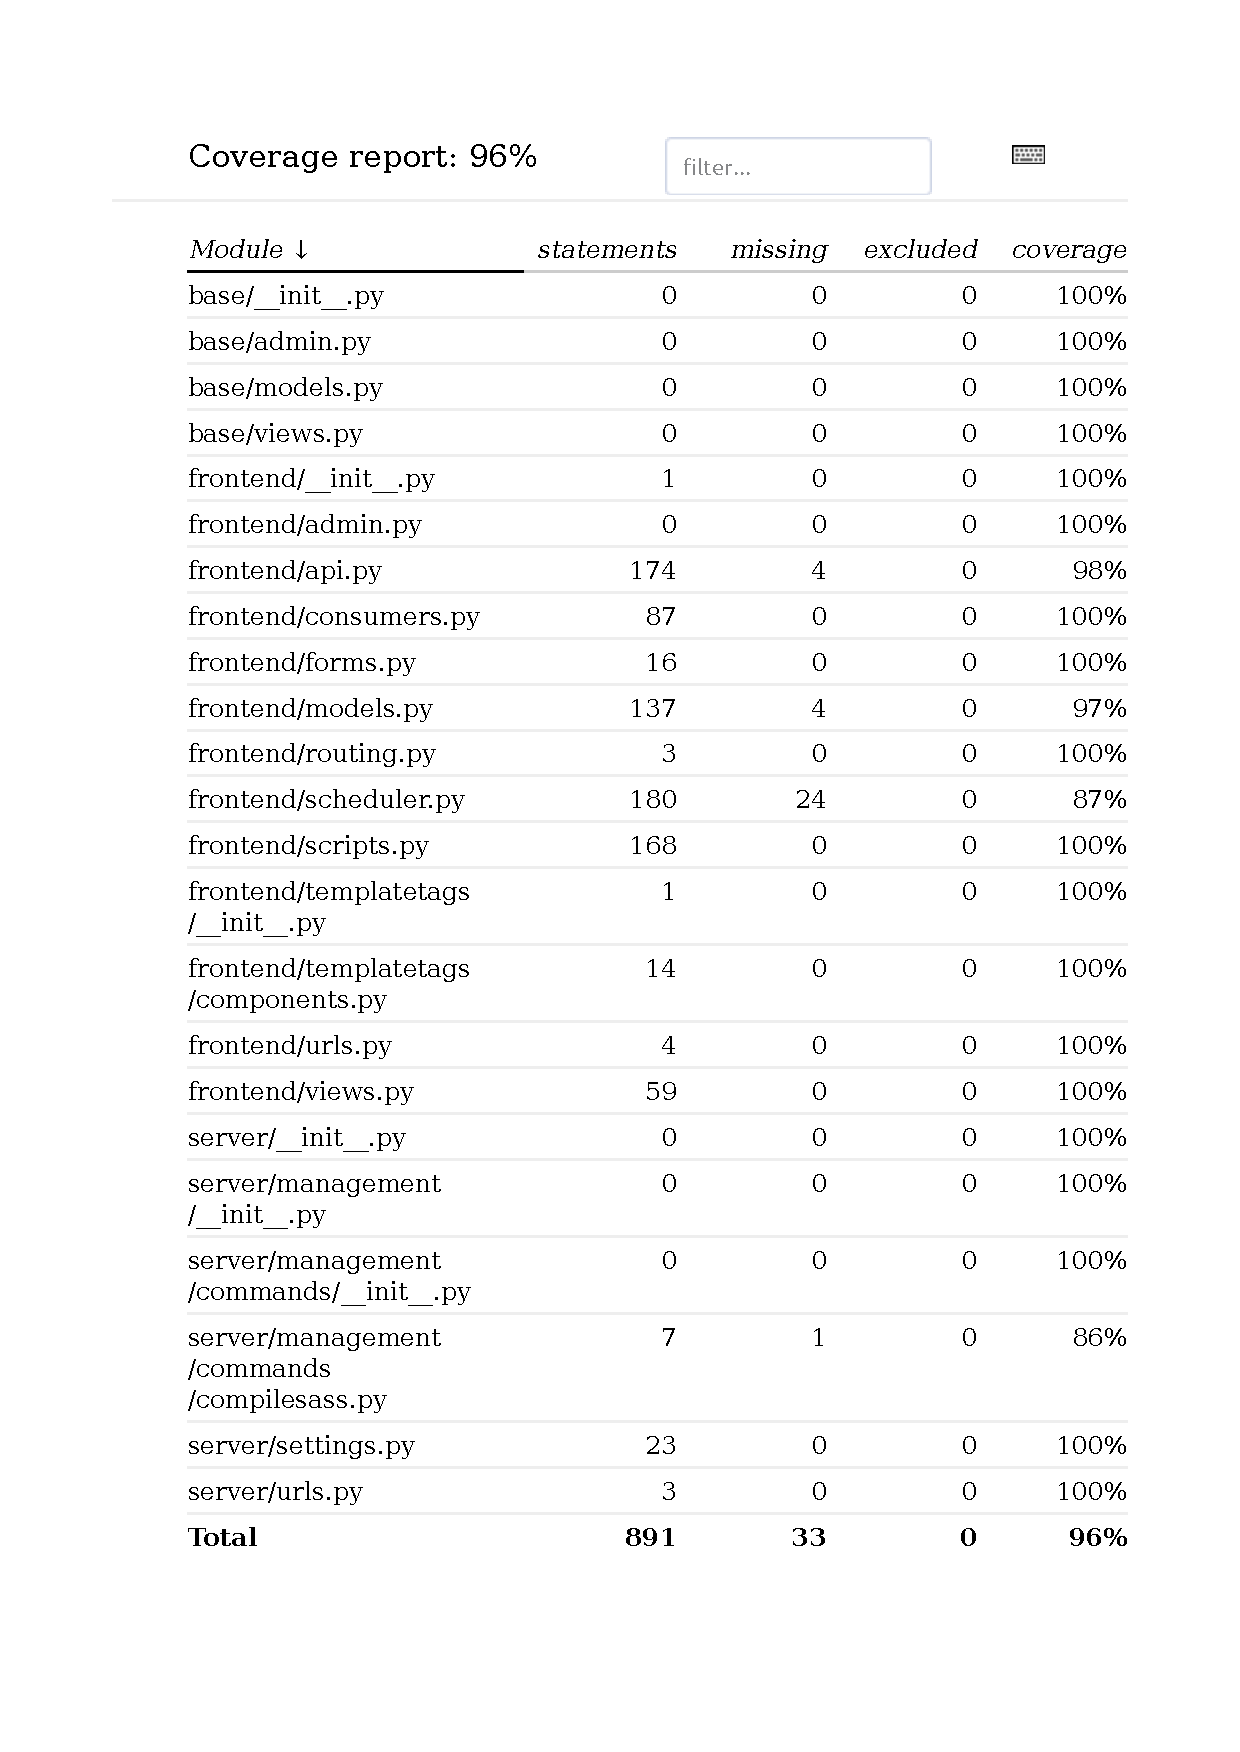
\includegraphics[width=.9\textwidth]{test_output/05_iteration_coverage.pdf}
	\caption{Coverage in Iteration 5}
\end{figure}

\subsubsection{6. Iteration}
\begin{table}[H]
\begin{center}
	\begin{tabular}{| l | l |}
		\hline
		\textbf{Zeitraum} &  05.02.2018 - 18.02.2018\\\hline
		\textbf{Abgegebene Userstorys} & keine\\\hline
		\textbf{Commit Hash} & - \\\hline
	\end{tabular}
	\caption{Übersicht 6. Iteration}
\end{center}
\end{table}
In dieser Iteration wurden alle Userstorys von den Auftraggebern abgelehnt und wurden daher in der nächsten Iteration mit
den angemerkten Änderungen neu eingereicht.

\subsubsection{7. Iteration}
\begin{table}[H]
\begin{center}
	\begin{tabular}{| l | l |}
		\hline
		\textbf{Zeitraum} &  19.02.2018 - 04.03.2018\\\hline
		\textbf{Abgegebene Userstorys} & 9,26,30,37,38,39,40\\\hline
		\textbf{Commit Hash} & \texttt{6003099c26804bff6995ac4ff0d0d5571dfc2840} \\\hline
	\end{tabular}
	\caption{Übersicht 7. Iteration}
\end{center}
\end{table}
\subsubsection{Testoutput }
\lstinputlisting{test_output/07_iteration_python}
\subsubsection{Coverage}
\begin{figure}[H]
	\centering
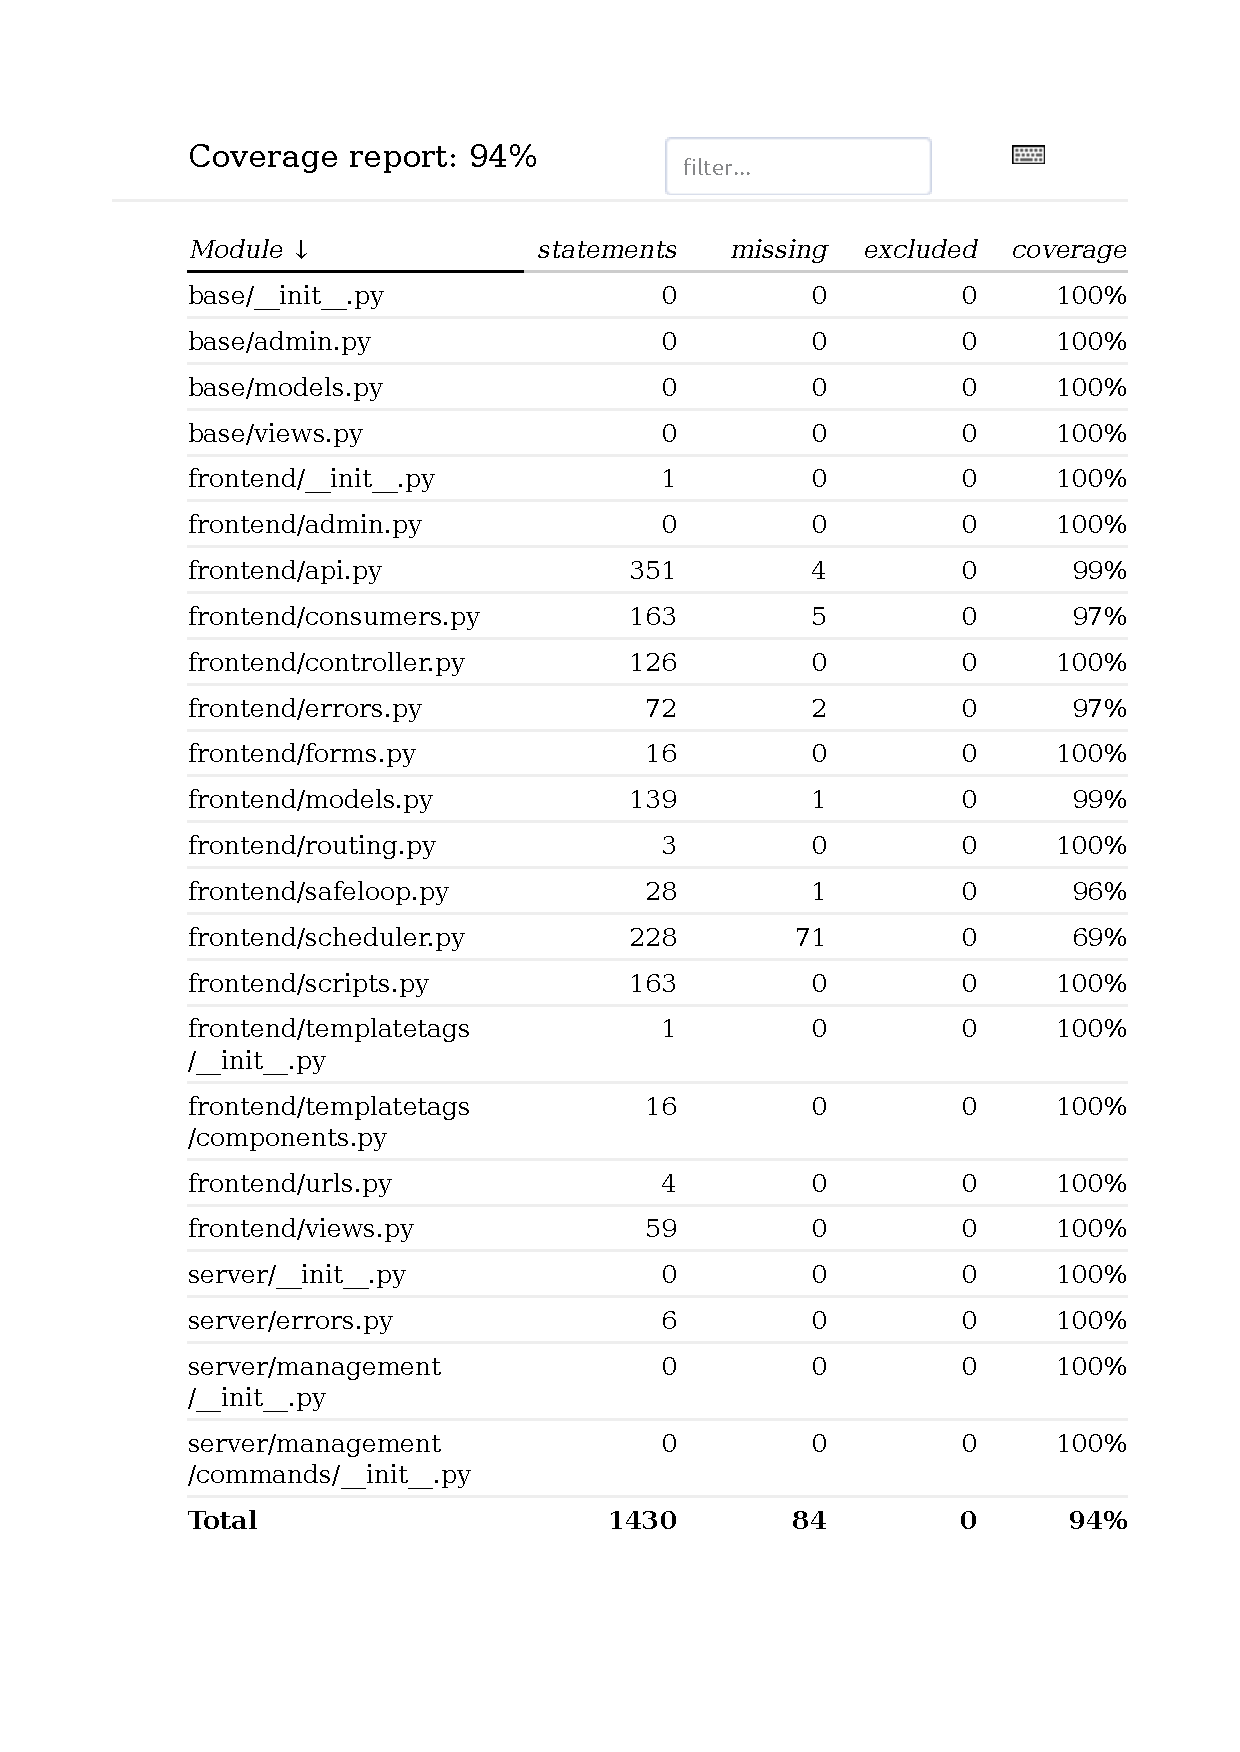
\includegraphics[width=.9\textwidth]{test_output/07_iteration_coverage.pdf}
	\caption{Coverage in Iteration 7}
\end{figure}

\subsubsection{8. Iteration}
\begin{table}[H]
\begin{center}
	\begin{tabular}{| l | l |}
		\hline
		\textbf{Zeitraum} &  05.03.2018 - 18.03.2018\\\hline
		\textbf{Abgegebene Userstorys} & 41, 45\\\hline
		\textbf{Commit Hash} & \texttt{13351d683a279c48b2890d23add9bfa57963fea8} \\\hline
	\end{tabular}
	\caption{Übersicht 8. Iteration}
\end{center}
\end{table}
\subsubsection{Testoutput }
\lstinputlisting{test_output/08_iteration_python}
\subsubsection{Coverage}
\begin{figure}[H]
	\centering
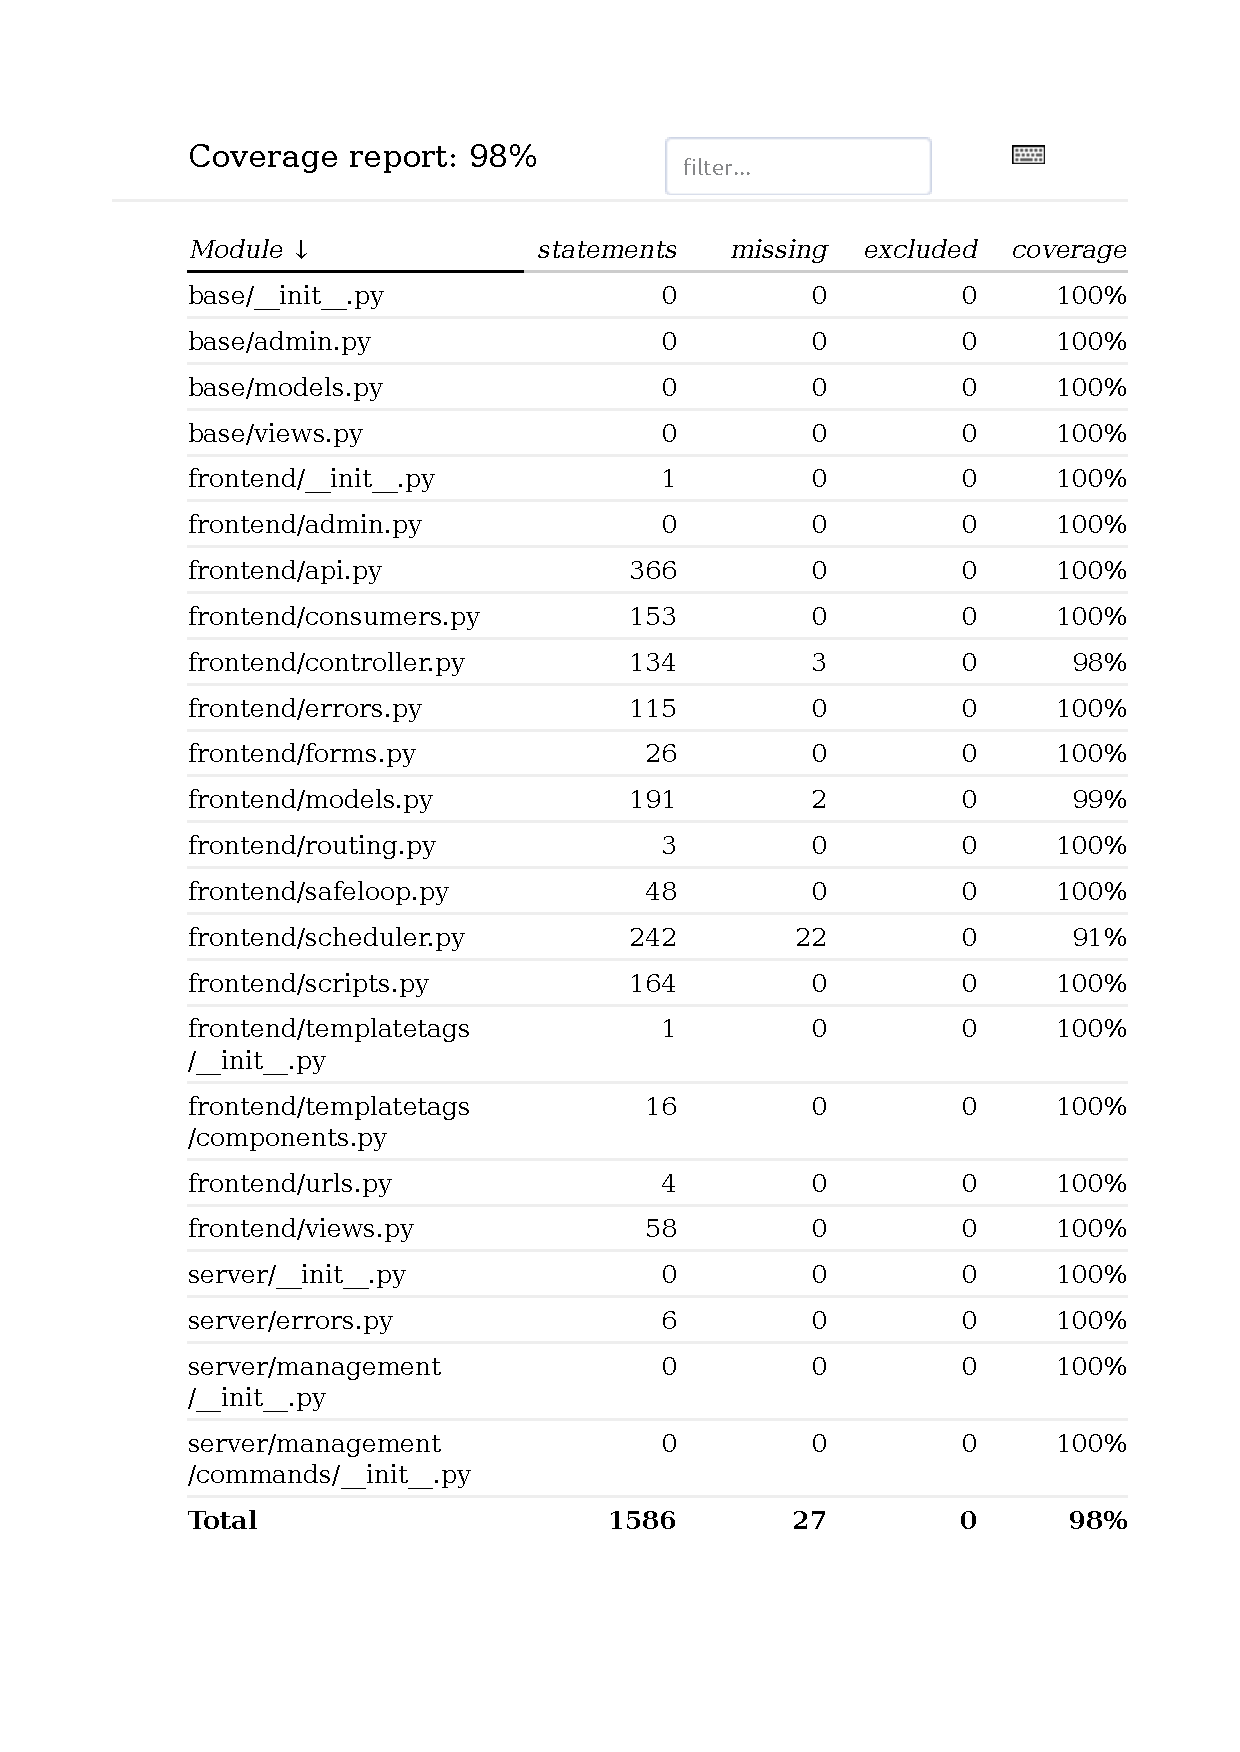
\includegraphics[width=.9\textwidth]{test_output/08_iteration_coverage.pdf}
	\caption{Coverage in Iteration 8}
\end{figure}

\subsubsection{9. Iteration}
\begin{table}[H]
\begin{center}
	\begin{tabular}{| l | l |}
		\hline
		\textbf{Zeitraum} &  19.03.2018 - 28.03.2018\\\hline
		\textbf{Abgegebene Userstorys} & 32, 42, 43, 44, 46, 47, 48\\\hline
		\textbf{Commit Hash} & \texttt{459b7edca36d0602017a1d724e2f159ce544aa1d} \\\hline
	\end{tabular}
	\caption{Übersicht 9. Iteration}
\end{center}
\end{table}
\subsubsection{Testoutput }
\lstinputlisting{test_output/09_iteration_python}
\subsubsection{Coverage}
\begin{figure}[H]
	\centering
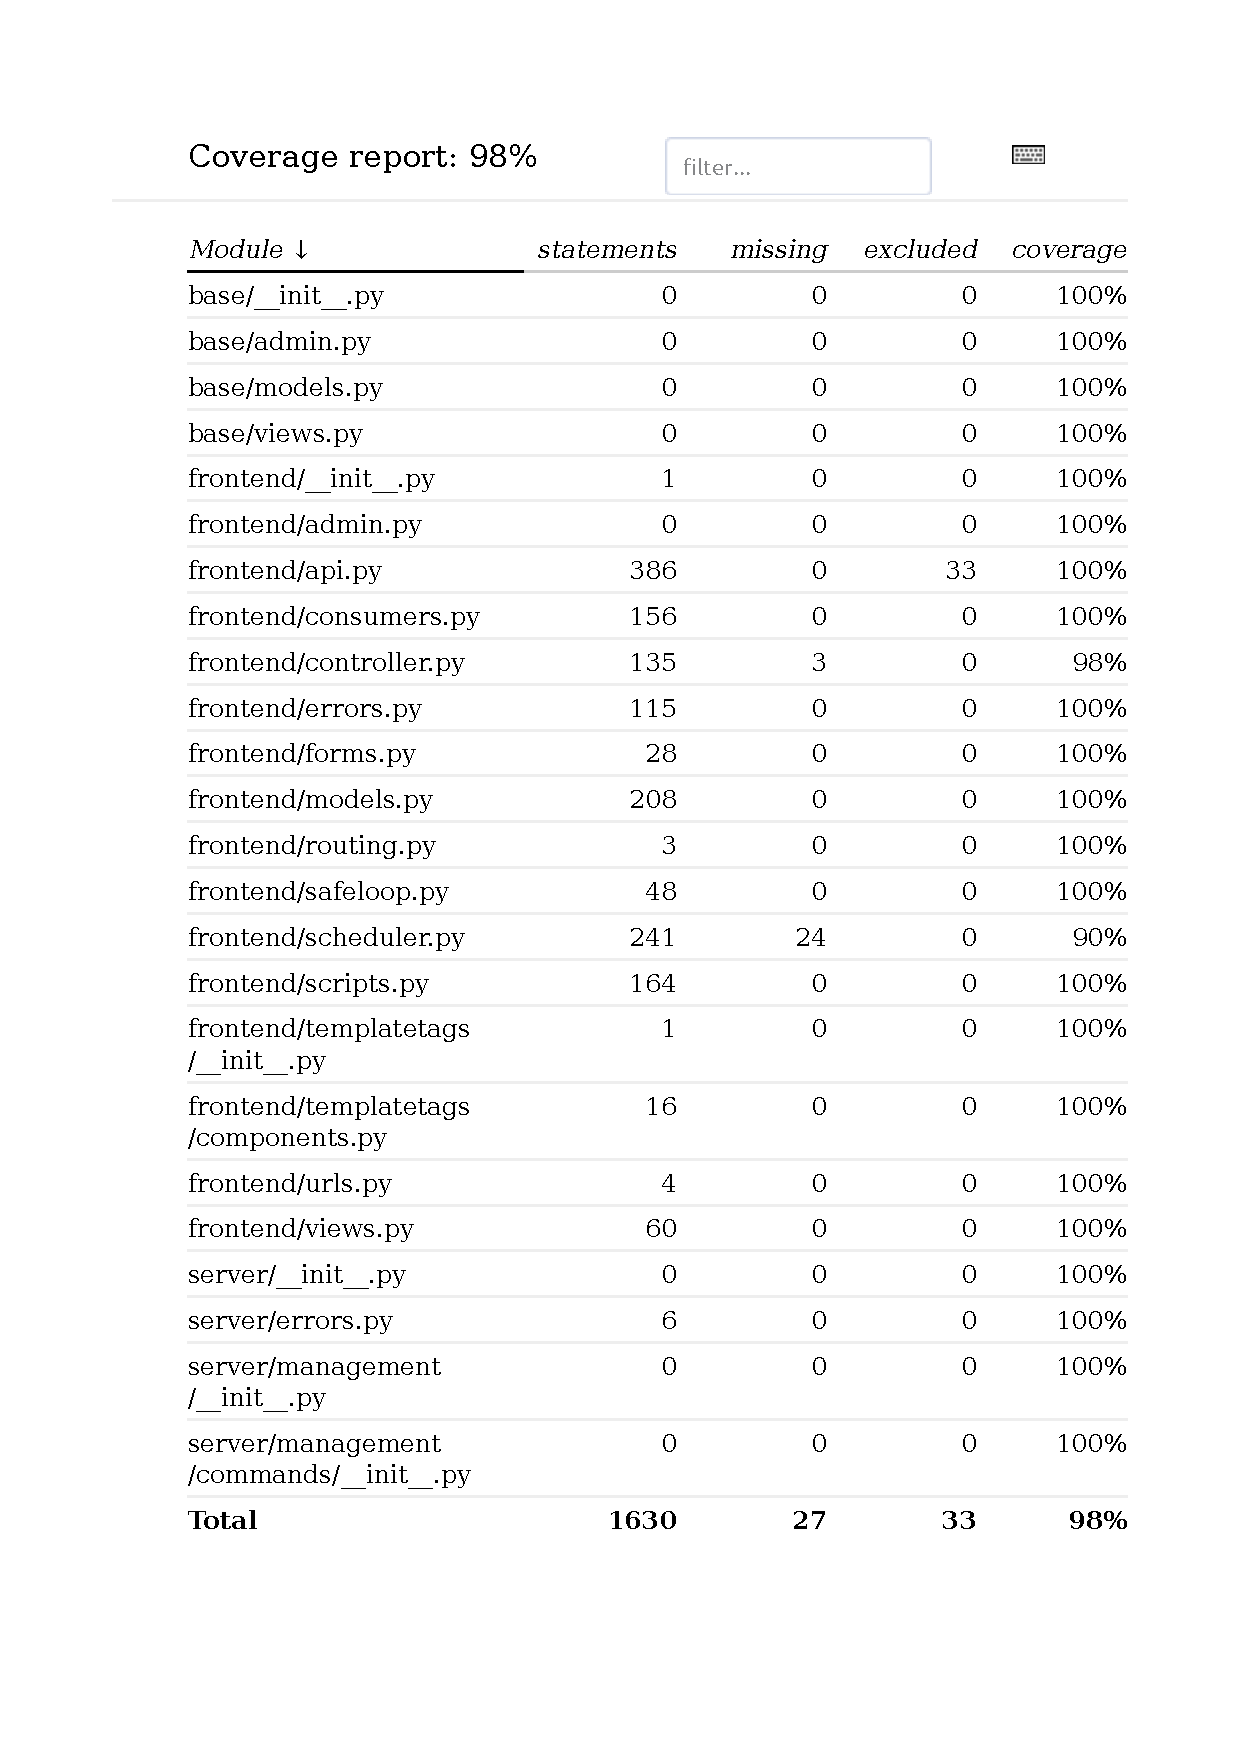
\includegraphics[width=.9\textwidth]{test_output/09_iteration_coverage.pdf}
	\caption{Coverage in Iteration 9}
\end{figure}

	% Ausgefüllte Code Reviews
	\section{Code Reviews}
Nach der Implementierung einer Userstory mussten alle Änderungen am Code von einem weiteren Entwickler
gesichtet werden. Dabei wurde folgende Checkliste als Referenz verwendet:
\begin{itemize}
	\item Test Coverage (auf unseren Dateien) mindestens 90\%
	\item Jede Klasse und Funktion ist grob Dokumentiert
	\item Schwierige Codestellen sind dokumentiert
	\item Alle Test laufen fehlerfrei durch
	\item Der Code ist korrekt formatiert
	\item Code erfüllt das Akzeptanzkriterium der Userstory (und dabei spezifisch nur das Akzeptanzkriterium dieser Userstory)
	\item Die Userstory ist ausgefüllt (Datum, Zeit)
\end{itemize}
Es folgen die ausgefüllten Checklisten. Da die ersten beiden US in gemeinsamer Arbeit entstanden ist, gibt es keine Checkliste dafür.
\begin{figure}[H]
\centering
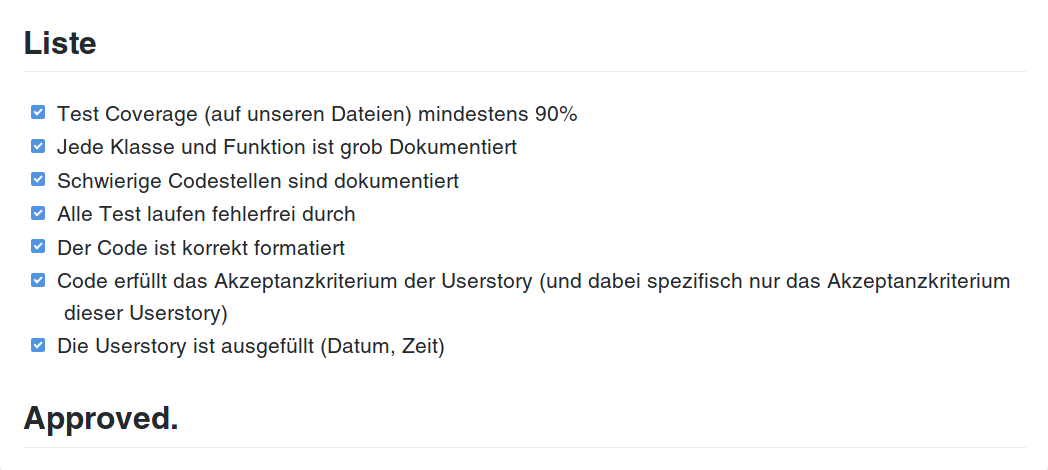
\includegraphics[width=.8\textwidth]{code_review/us03}
	\caption{Review zur Userstory 3}
\end{figure}

\begin{figure}[H]
\centering
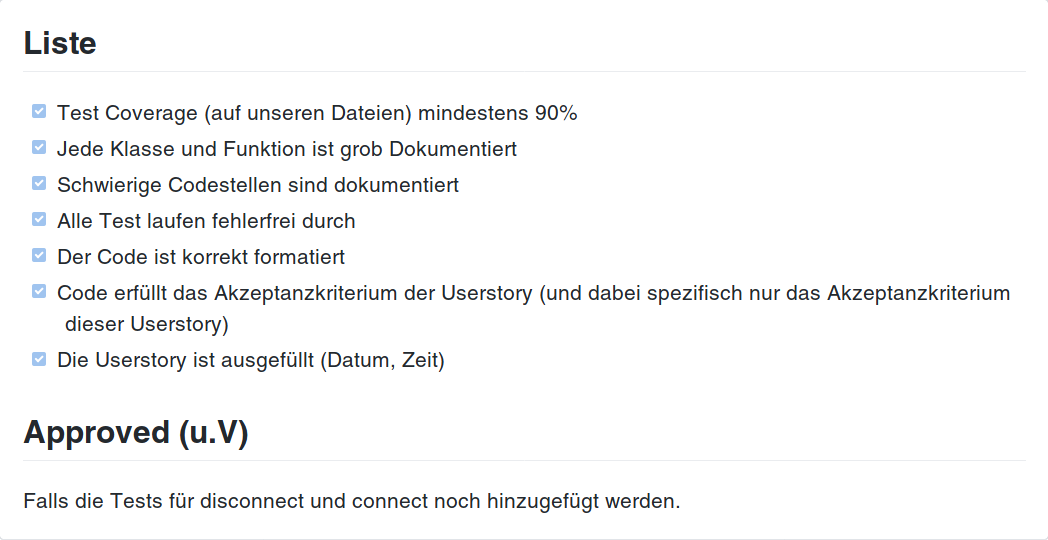
\includegraphics[width=.8\textwidth]{code_review/us04}
\caption{Review zur Userstory 04}
\end{figure}

\begin{figure}[H]
\centering
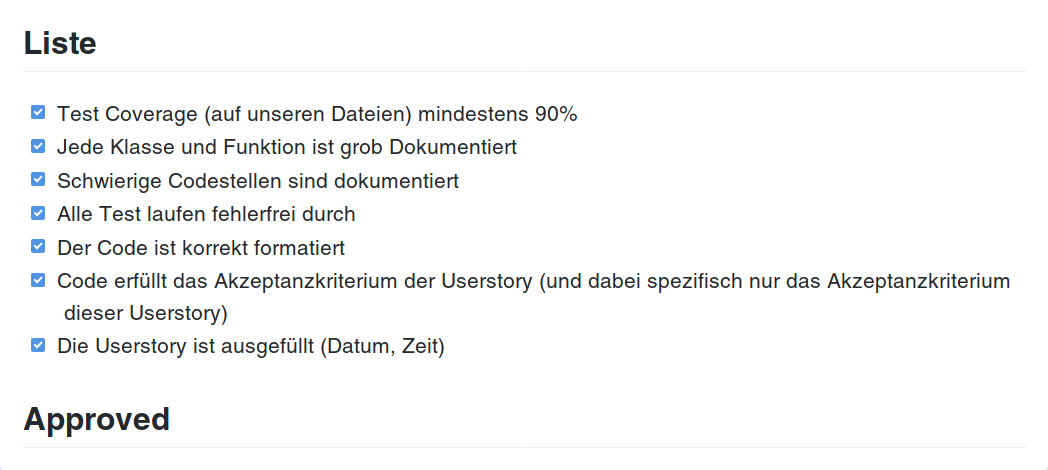
\includegraphics[width=.8\textwidth]{code_review/us05}
\caption{Review zur Userstory 05}
\end{figure}

\begin{figure}[H]
\centering
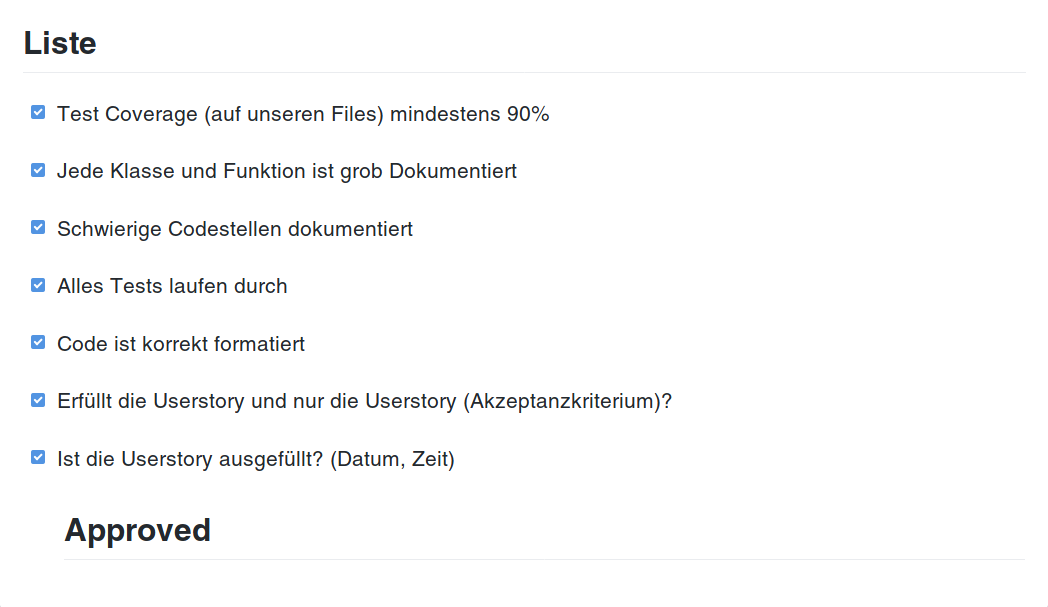
\includegraphics[width=.8\textwidth]{code_review/us06}
\caption{Review zur Userstory 06}
\end{figure}

\begin{figure}[H]
\centering
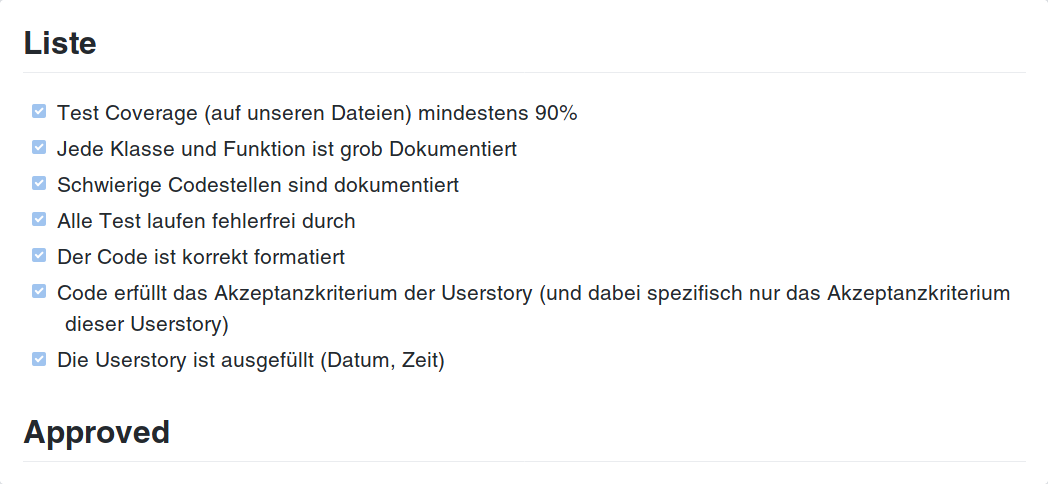
\includegraphics[width=.8\textwidth]{code_review/us07}
\caption{Review zur Userstory 07}
\end{figure}

\begin{figure}[H]
\centering
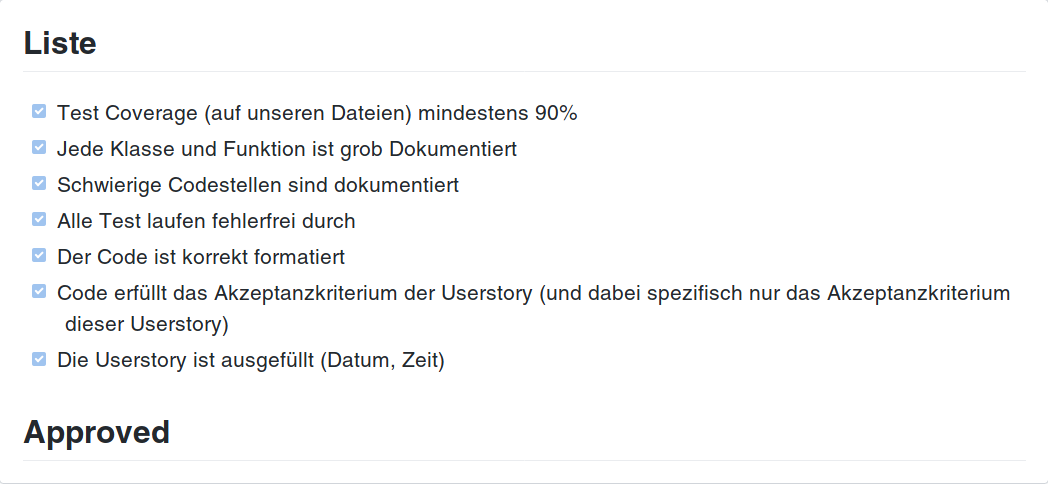
\includegraphics[width=.8\textwidth]{code_review/us08}
\caption{Review zur Userstory 08}
\end{figure}

\begin{figure}[H]
\centering
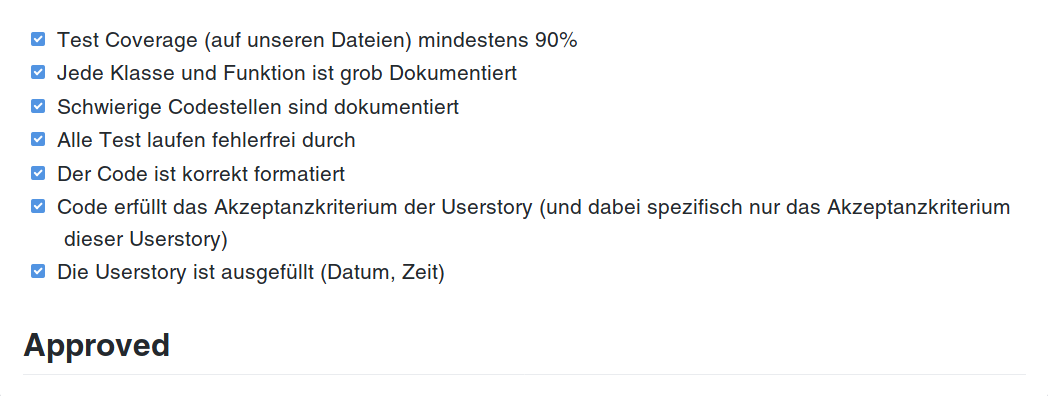
\includegraphics[width=.8\textwidth]{code_review/us09}
\caption{Review zur Userstory 09}
\end{figure}

\begin{figure}[H]
\centering
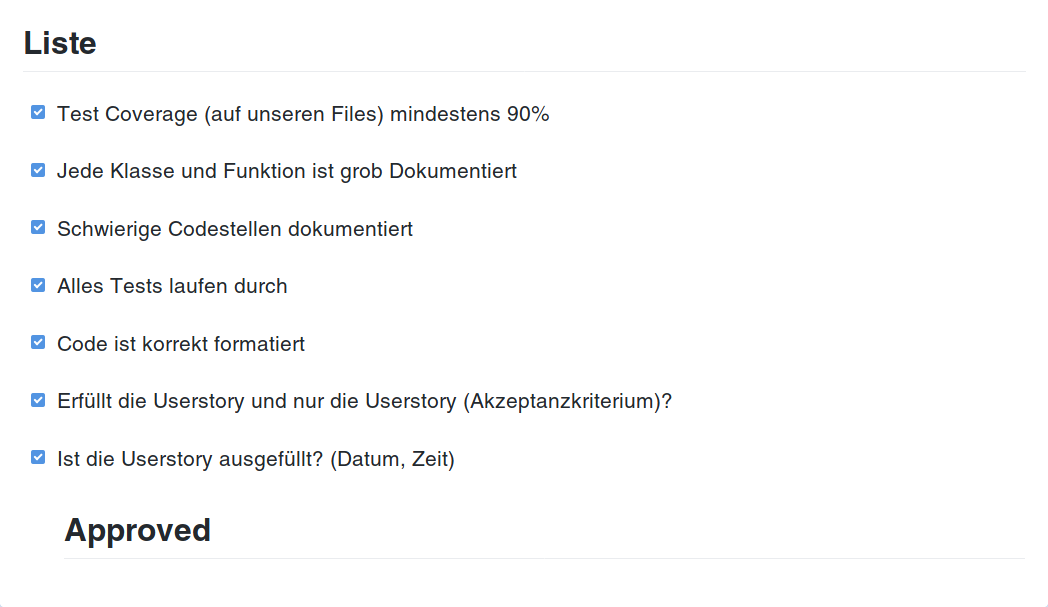
\includegraphics[width=.8\textwidth]{code_review/us14}
\caption{Review zur Userstory 14}
\end{figure}

\begin{figure}[H]
\centering
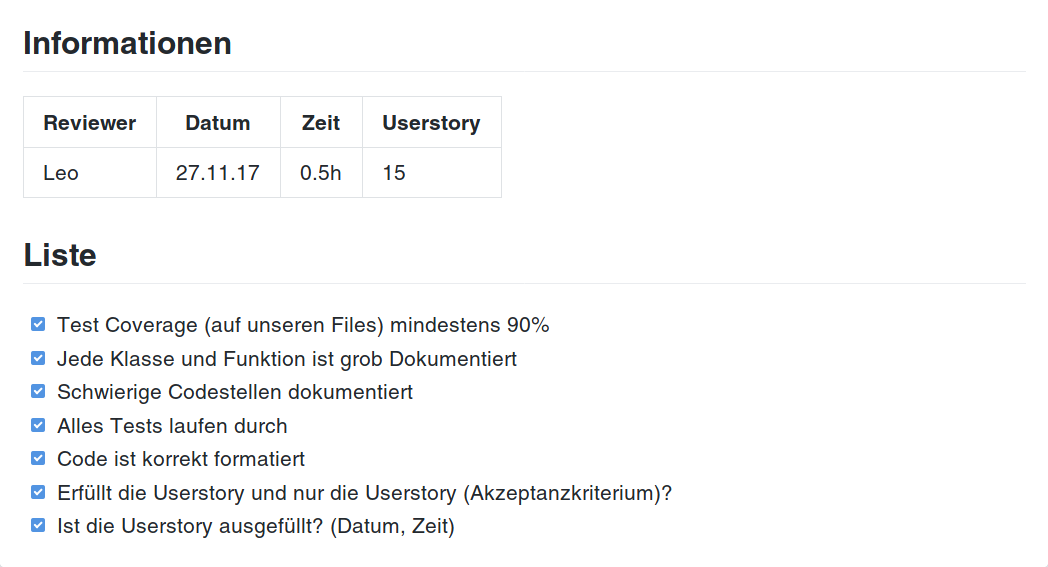
\includegraphics[width=.8\textwidth]{code_review/us15}
\caption{Review zur Userstory 15}
\end{figure}

\begin{figure}[H]
\centering
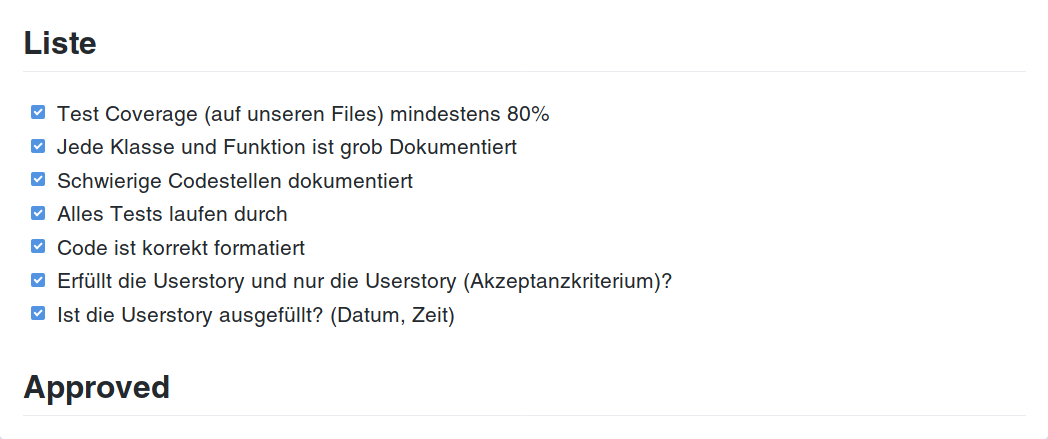
\includegraphics[width=.8\textwidth]{code_review/us16}
\caption{Review zur Userstory 16}
\end{figure}

\begin{figure}[H]
\centering
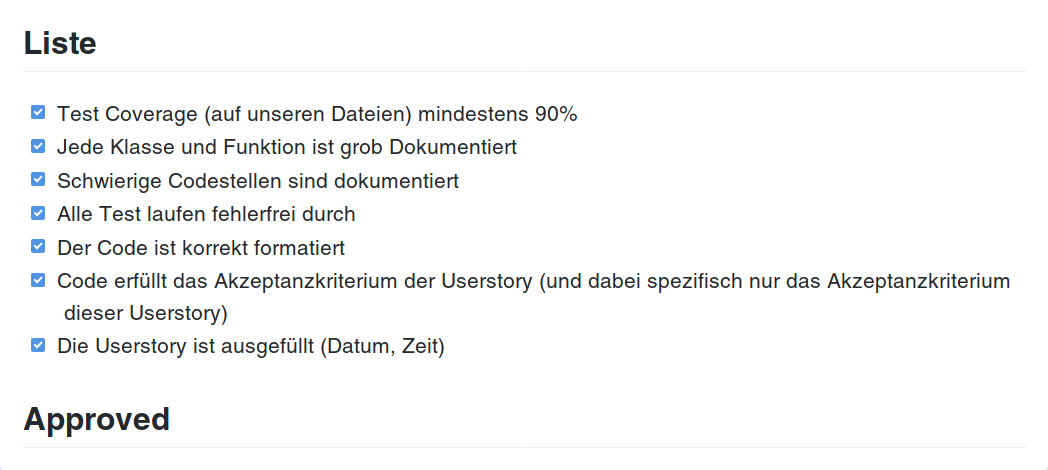
\includegraphics[width=.8\textwidth]{code_review/us17}
\caption{Review zur Userstory 17}
\end{figure}

\begin{figure}[H]
\centering
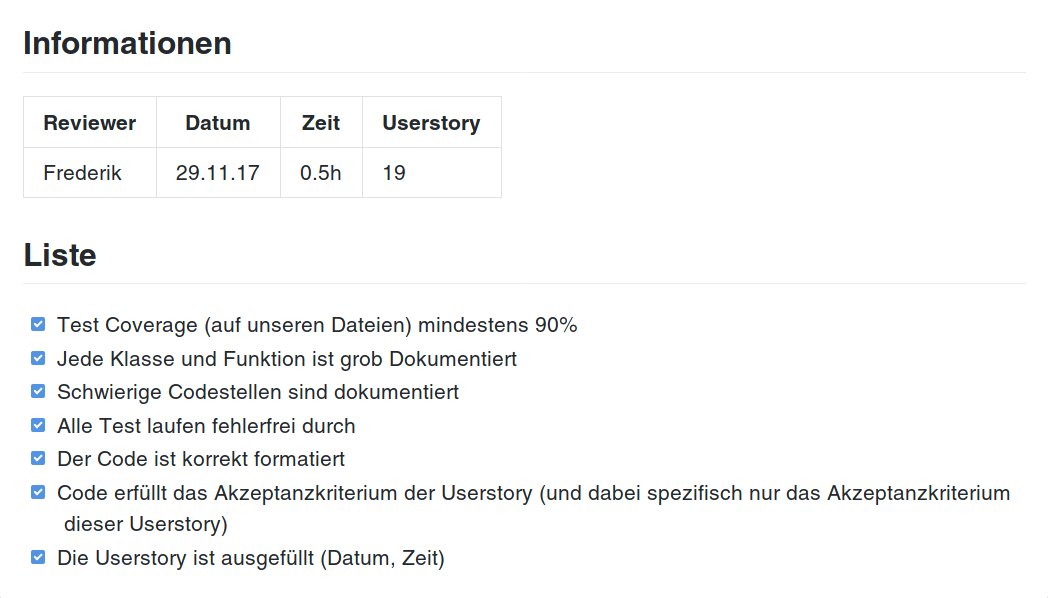
\includegraphics[width=.8\textwidth]{code_review/us19}
\caption{Review zur Userstory 19}
\end{figure}

\begin{figure}[H]
\centering
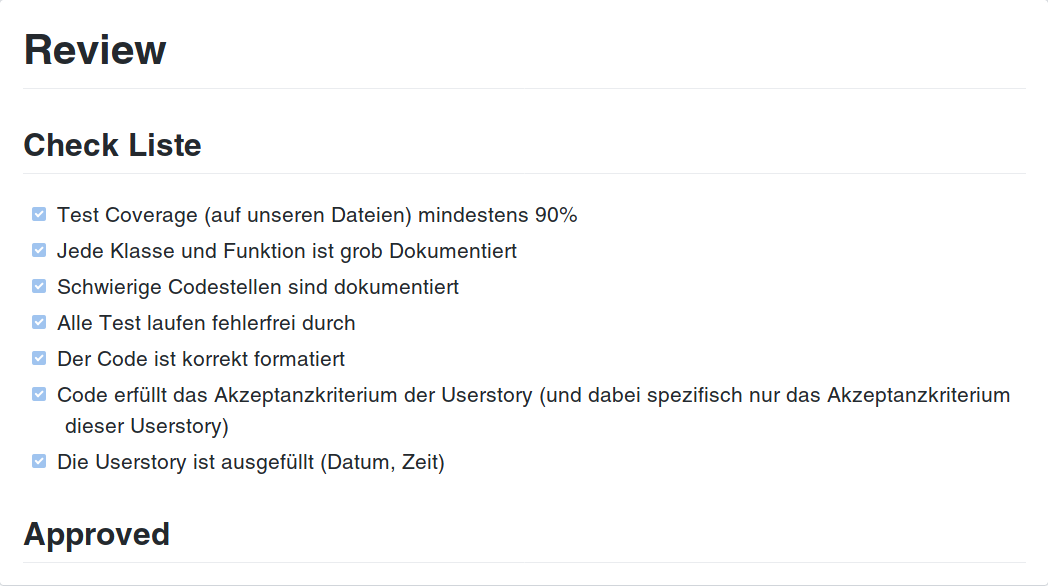
\includegraphics[width=.8\textwidth]{code_review/us20}
\caption{Review zur Userstory 20}
\end{figure}

\begin{figure}[H]
\centering
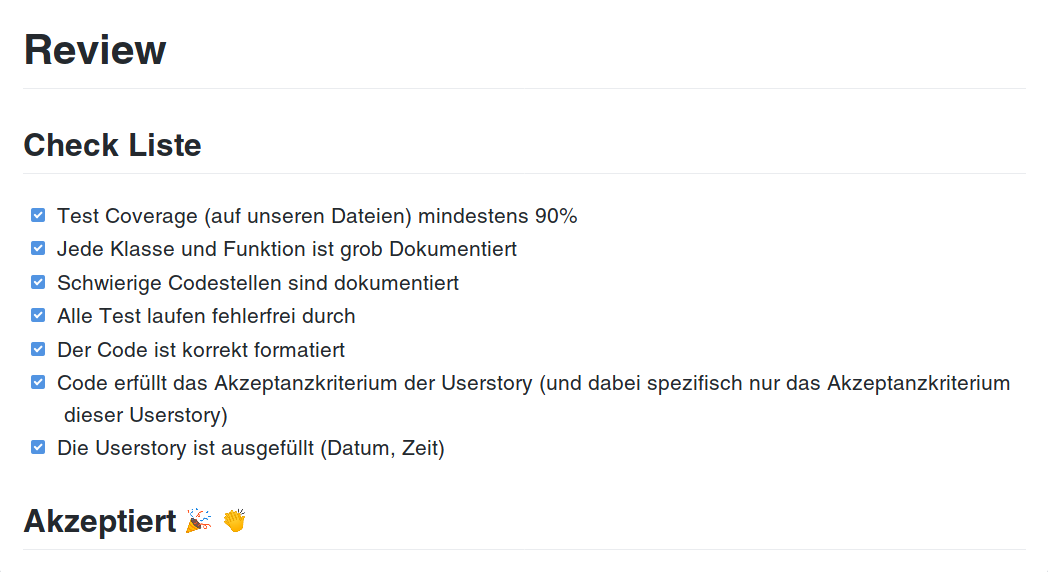
\includegraphics[width=.8\textwidth]{code_review/us21}
\caption{Review zur Userstory 21}
\end{figure}

\begin{figure}[H]
\centering
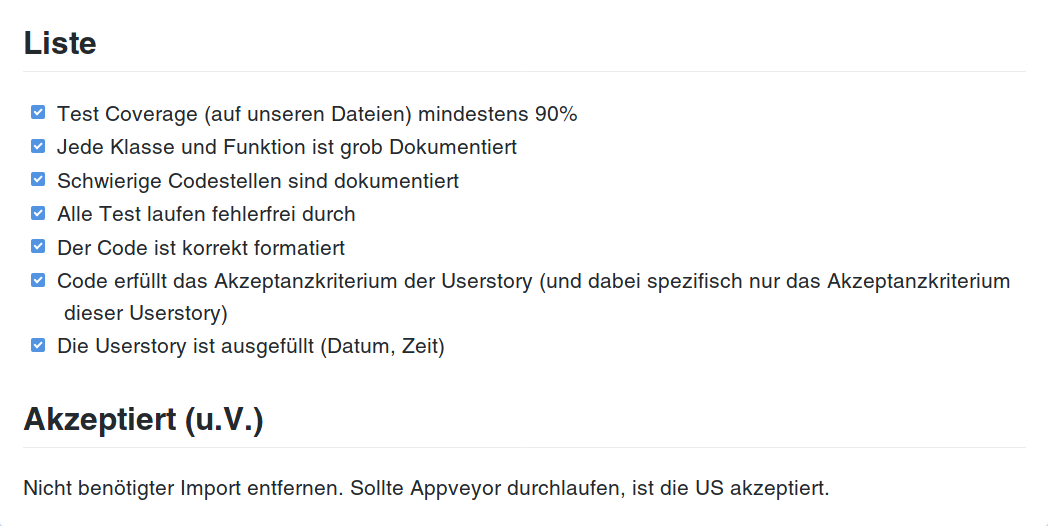
\includegraphics[width=.8\textwidth]{code_review/us22}
\caption{Review zur Userstory 22}
\end{figure}

\begin{figure}[H]
\centering
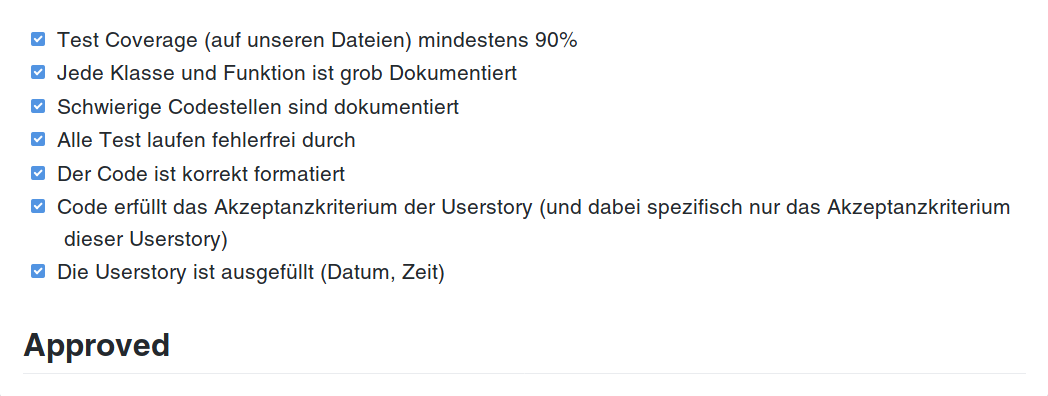
\includegraphics[width=.8\textwidth]{code_review/us23}
\caption{Review zur Userstory 23}
\end{figure}

\begin{figure}[H]
\centering
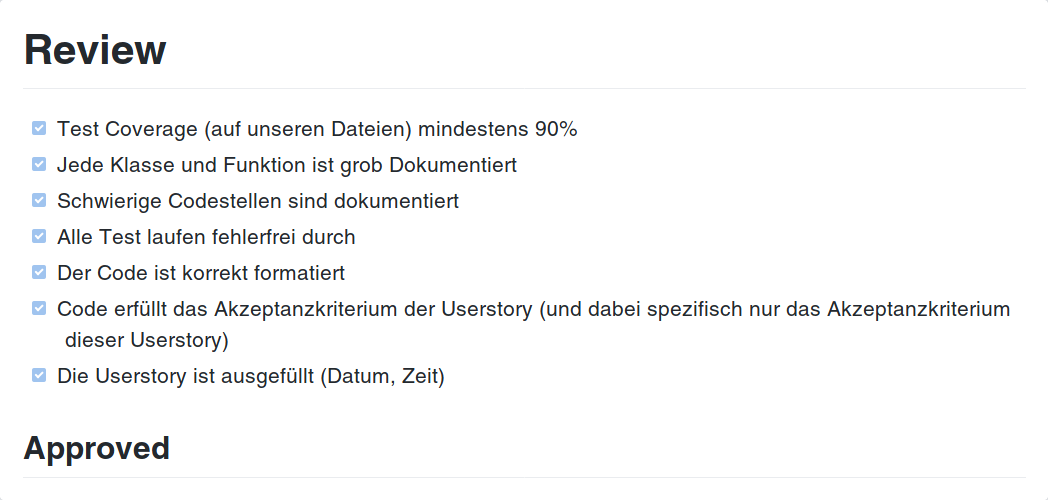
\includegraphics[width=.8\textwidth]{code_review/us24}
\caption{Review zur Userstory 24}
\end{figure}

\begin{figure}[H]
\centering
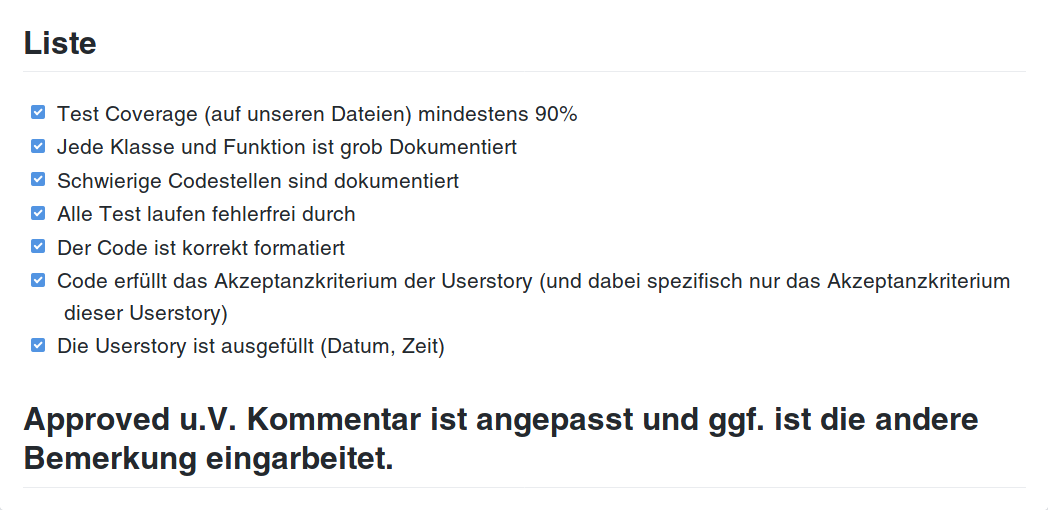
\includegraphics[width=.8\textwidth]{code_review/us25}
\caption{Review zur Userstory 25}
\end{figure}

\begin{figure}[H]
\centering
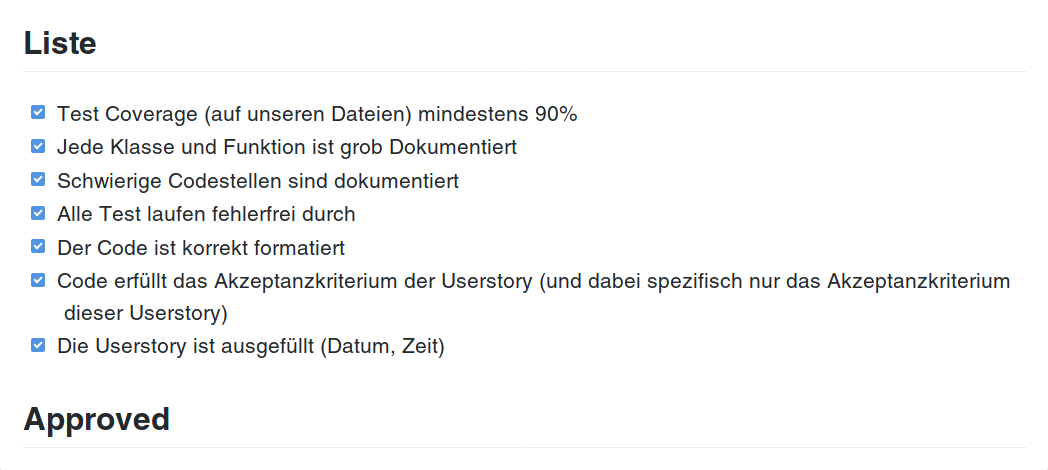
\includegraphics[width=.8\textwidth]{code_review/us26}
\caption{Review zur Userstory 26}
\end{figure}

\begin{figure}[H]
\centering
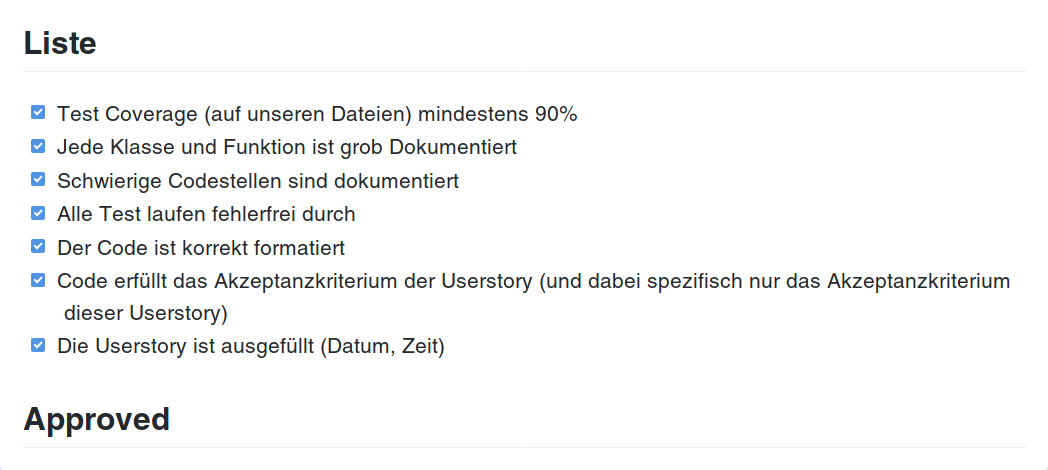
\includegraphics[width=.8\textwidth]{code_review/us27}
\caption{Review zur Userstory 27}
\end{figure}

\begin{figure}[H]
\centering
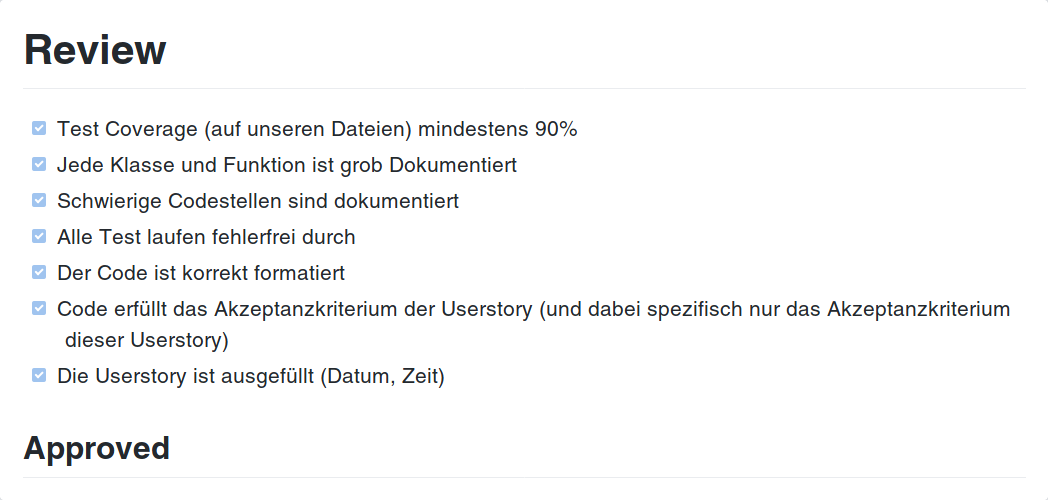
\includegraphics[width=.8\textwidth]{code_review/us28}
\caption{Review zur Userstory 28}
\end{figure}

\begin{figure}[H]
\centering
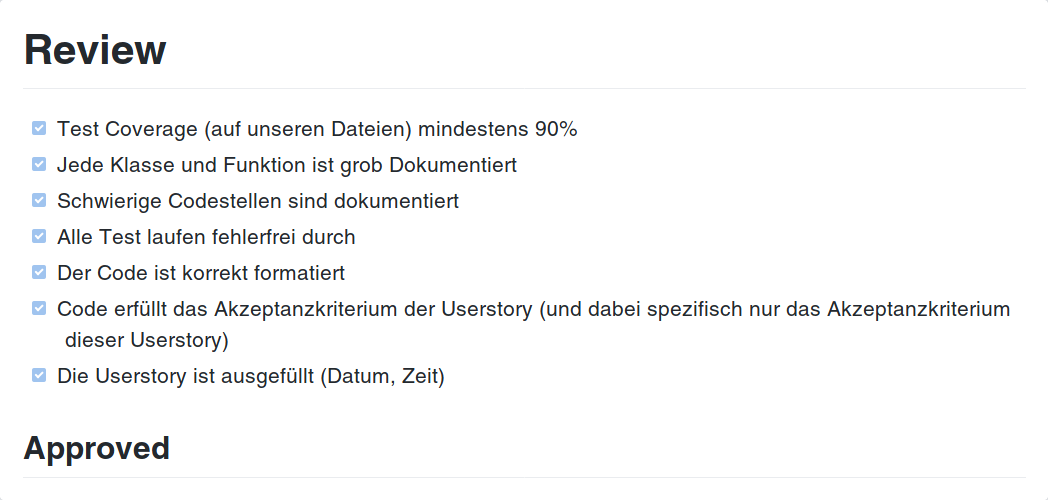
\includegraphics[width=.8\textwidth]{code_review/us29}
\caption{Review zur Userstory 29}
\end{figure}

\begin{figure}[H]
\centering
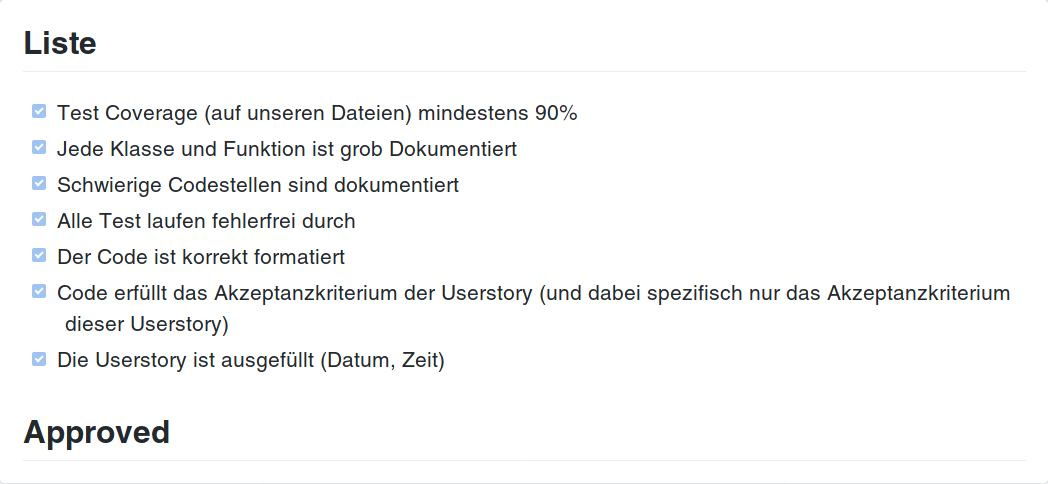
\includegraphics[width=.8\textwidth]{code_review/us30}
\caption{Review zur Userstory 30}
\end{figure}

\begin{figure}[H]
\centering
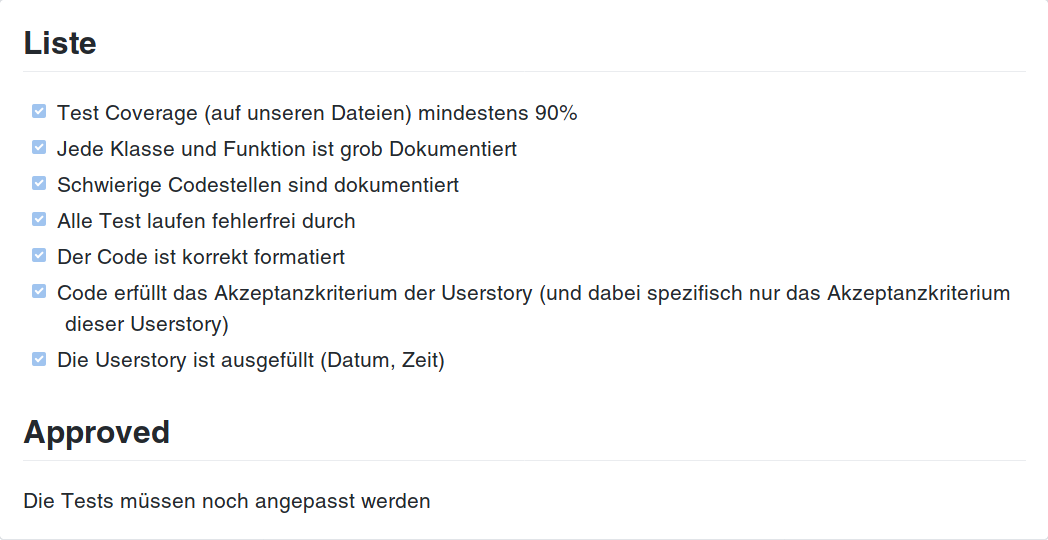
\includegraphics[width=.8\textwidth]{code_review/us31}
\caption{Review zur Userstory 31}
\end{figure}

\begin{figure}[H]
\centering
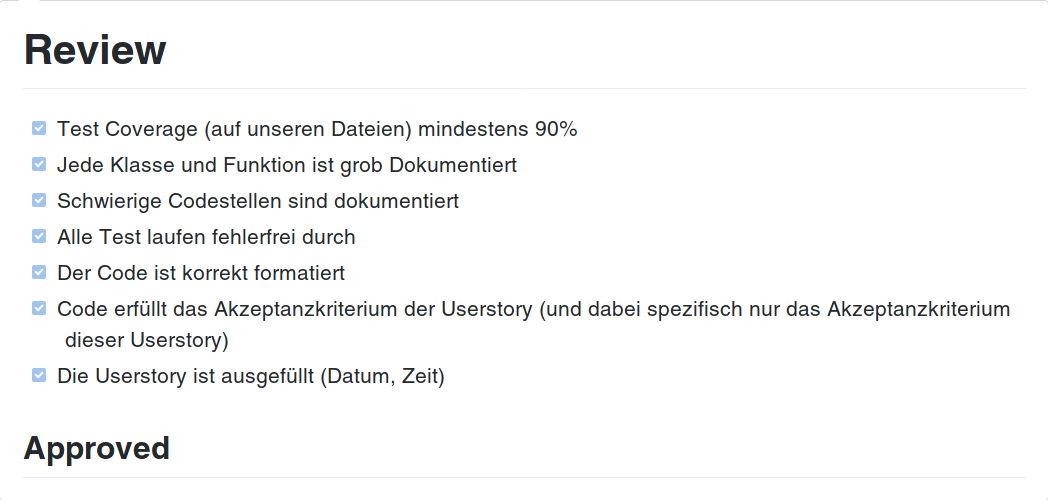
\includegraphics[width=.8\textwidth]{code_review/us32}
\caption{Review zur Userstory 32}
\end{figure}

\begin{figure}[H]
\centering
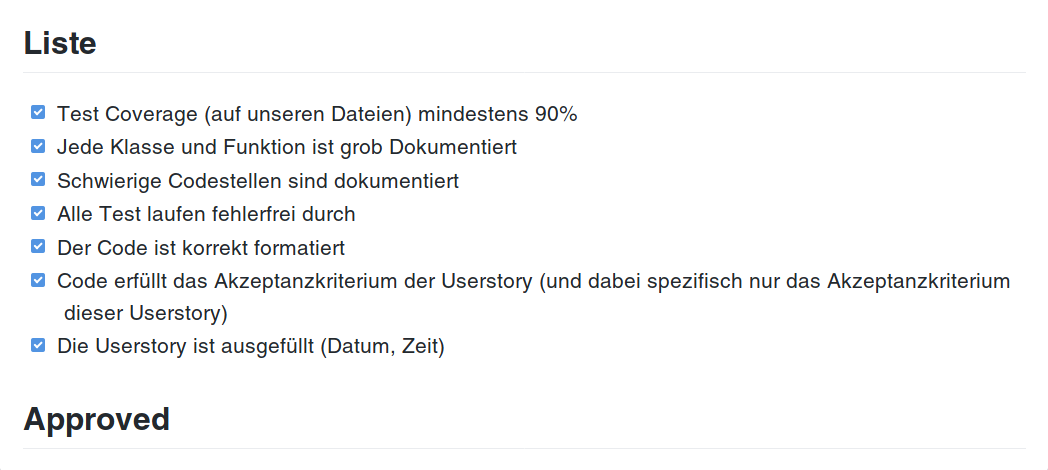
\includegraphics[width=.8\textwidth]{code_review/us33}
\caption{Review zur Userstory 33}
\end{figure}

\begin{figure}[H]
\centering
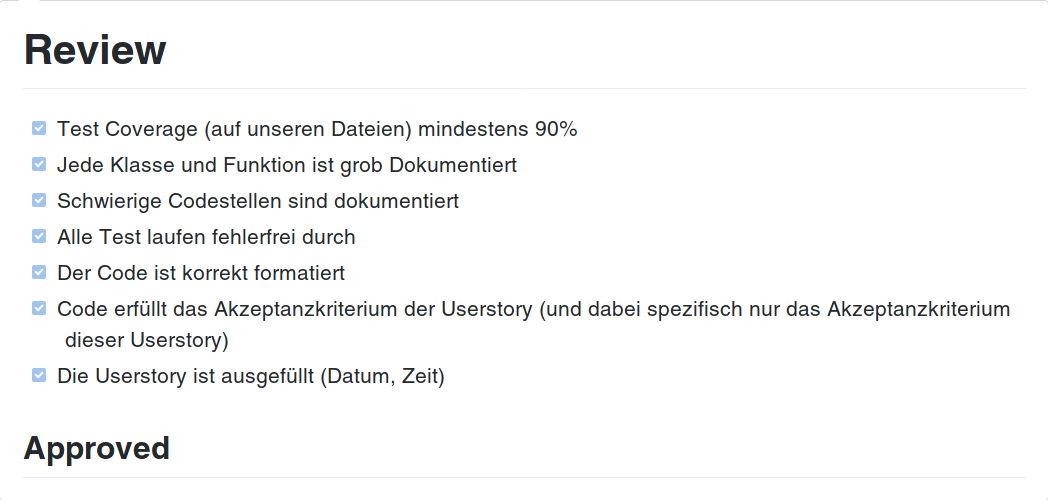
\includegraphics[width=.8\textwidth]{code_review/us34}
\caption{Review zur Userstory 34}
\end{figure}

\begin{figure}[H]
\centering
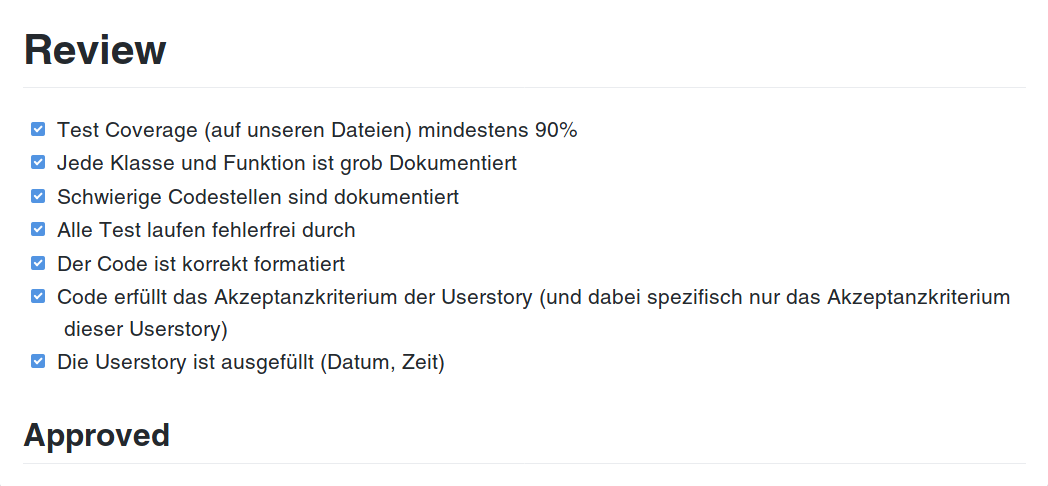
\includegraphics[width=.8\textwidth]{code_review/us35}
\caption{Review zur Userstory 35}
\end{figure}

\begin{figure}[H]
\centering
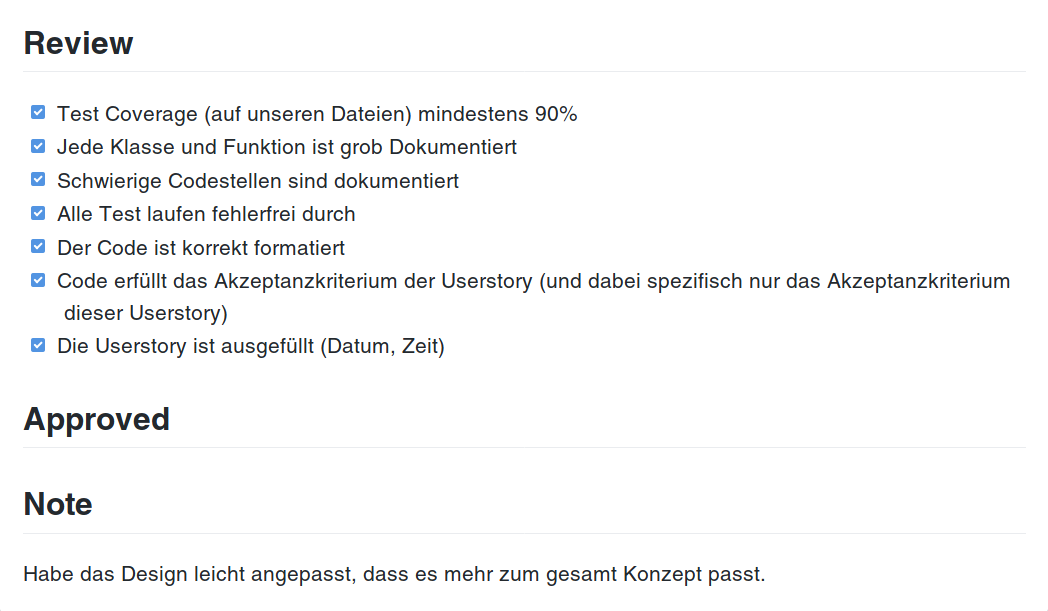
\includegraphics[width=.8\textwidth]{code_review/us36}
\caption{Review zur Userstory 36}
\end{figure}

\begin{figure}[H]
\centering
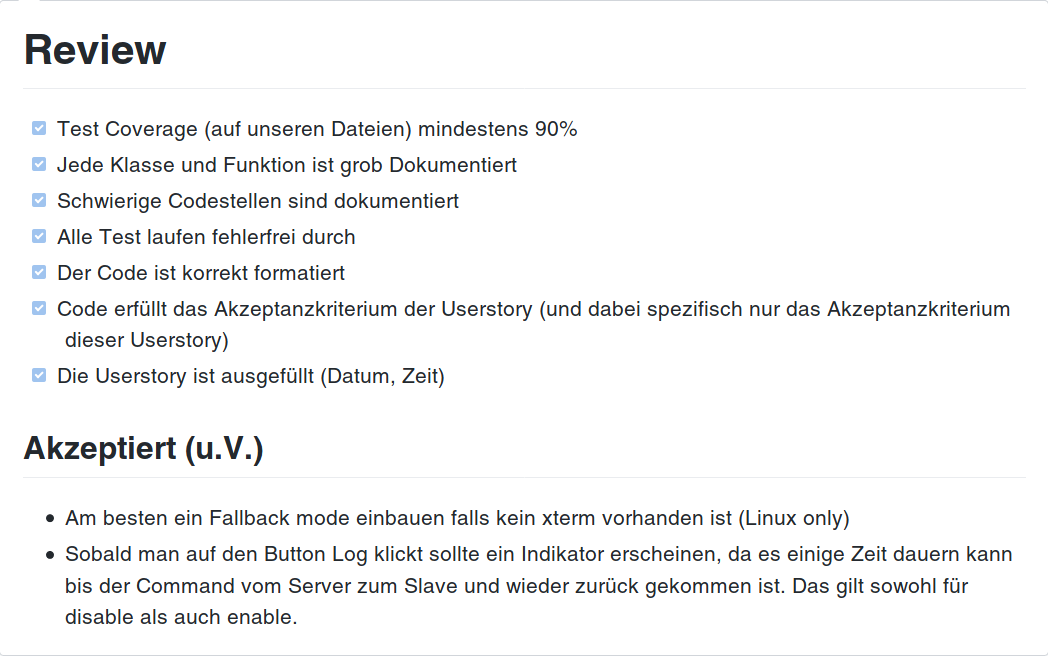
\includegraphics[width=.8\textwidth]{code_review/us37}
\caption{Review zur Userstory 37}
\end{figure}

\begin{figure}[H]
\centering
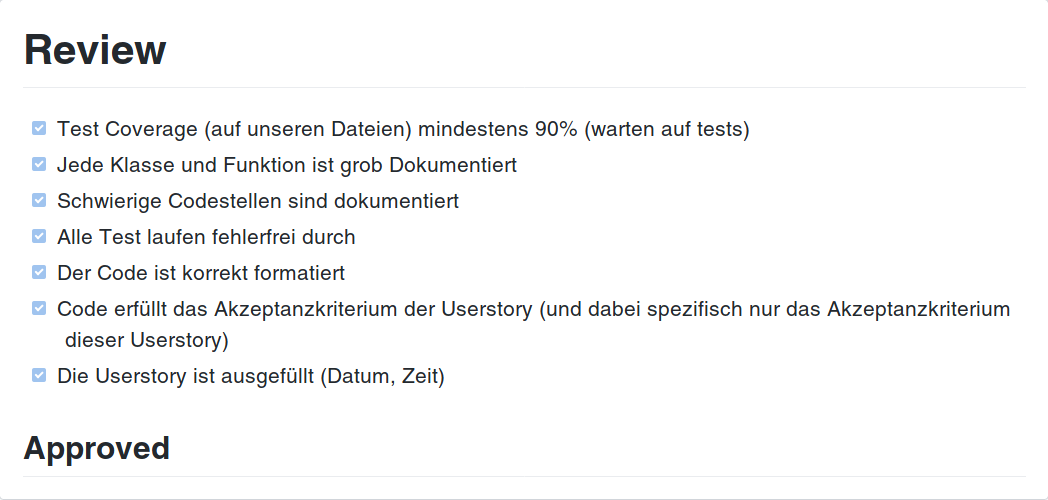
\includegraphics[width=.8\textwidth]{code_review/us38}
\caption{Review zur Userstory 38}
\end{figure}

\begin{figure}[H]
\centering
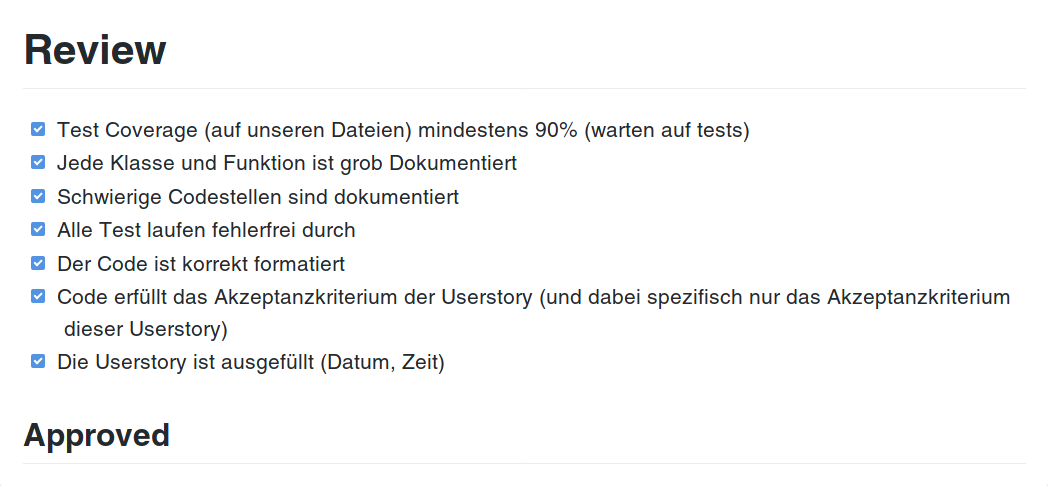
\includegraphics[width=.8\textwidth]{code_review/us39}
\caption{Review zur Userstory 39}
\end{figure}

\begin{figure}[H]
\centering
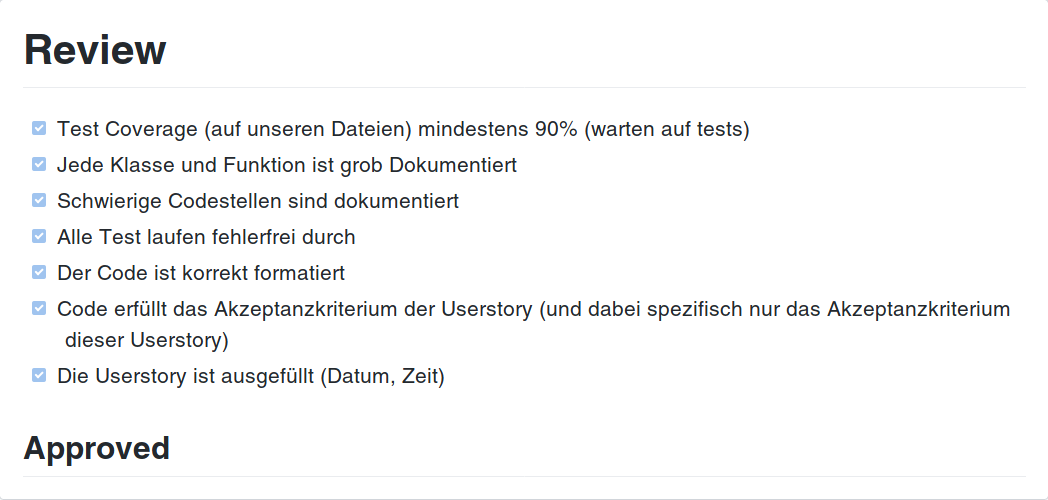
\includegraphics[width=.8\textwidth]{code_review/us40}
\caption{Review zur Userstory 40}
\end{figure}

\begin{figure}[H]
\centering
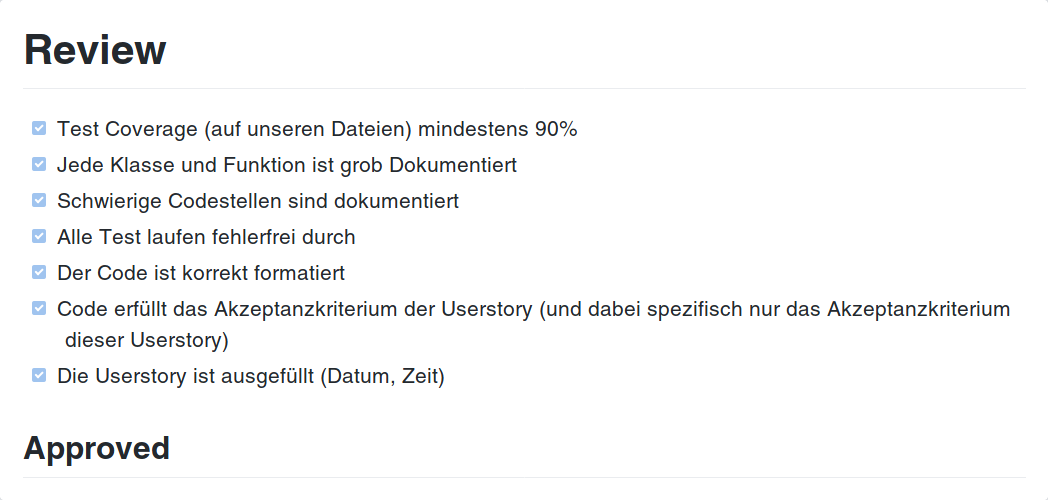
\includegraphics[width=.8\textwidth]{code_review/us41}
\caption{Review zur Userstory 41}
\end{figure}

\begin{figure}[H]
\centering
\includegraphics[width=.8\textwidth]{code_review/us42}
\caption{Review zur Userstory 42}
\end{figure}

\begin{figure}[H]
\centering
\includegraphics[width=.8\textwidth]{code_review/us43}
\caption{Review zur Userstory 43}
\end{figure}

\begin{figure}[H]
\centering
\includegraphics[width=.8\textwidth]{code_review/us44}
\caption{Review zur Userstory 44}
\end{figure}

\begin{figure}[H]
\centering
\includegraphics[width=.8\textwidth]{code_review/us45}
\caption{Review zur Userstory 45}
\end{figure}

\begin{figure}[H]
\centering
\includegraphics[width=.8\textwidth]{code_review/us46}
\caption{Review zur Userstory 46}
\end{figure}

\begin{figure}[H]
\centering
\includegraphics[width=.8\textwidth]{code_review/us47}
\caption{Review zur Userstory 47}
\end{figure}

\begin{figure}[H]
\centering
\includegraphics[width=.8\textwidth]{code_review/us48}
\caption{Review zur Userstory 48}
\end{figure}
\missingfigure{Restliche Reviews zu Userstorys hinzufügen}

	% Projekttagebuch
	\section{Projekttagebuch}
\subsection{Lizenz}
	Da sich die Auftraggeber eine größtmögliche Freiheit im Bezug
	auf die Verwendung des Codes gewünscht haben,
	wurde sämtlicher Code unter die MIT-Lizenz gestellt.
	\vspace{4em}
	\\\\
	MIT License
	\\\\
	Copyright (c) 2017 Frederik Bark, Heiko Carrasco, Jonas Meurer, Tim Weißmantel und Leonardo Zaninelli
	\\\\
	Permission is hereby granted, free of charge, to any person obtaining a copy of this software and associated documentation files (the ``Software''), to deal in the Software without restriction, including without limitation the rights to use, copy, modify, merge, publish, distribute, sublicense, and/or sell copies of the Software, and to permit persons to whom the Software is furnished to do so, subject to the following conditions:
	\\\\
	The above copyright notice and this permission notice shall be included in all copies or substantial portions of the Software.
	\\\\
	THE SOFTWARE IS PROVIDED ``AS IS'', WITHOUT WARRANTY OF ANY KIND, EXPRESS OR IMPLIED, INCLUDING BUT NOT LIMITED TO THE WARRANTIES OF MERCHANTABILITY, FITNESS FOR A PARTICULAR PURPOSE AND NONINFRINGEMENT. IN NO EVENT SHALL THE AUTHORS OR COPYRIGHT HOLDERS BE LIABLE FOR ANY CLAIM, DAMAGES OR OTHER LIABILITY, WHETHER IN AN ACTION OF CONTRACT, TORT OR OTHERWISE, ARISING FROM, OUT OF OR IN CONNECTION WITH THE SOFTWARE OR THE USE OR OTHER DEALINGS IN THE SOFTWARE.

	
\subsection{Projektgefährdende Ereignisse}
\textit{keine}



\end{document}
